%  LaTeX support: latex@mdpi.com
%  Template: MDPI Systems journal (ISSN 2079-8954), class from ihrke/mdpi (11 March 2023 mdpi.cls)
\documentclass[systems,article,submit,moreauthors,pdftex,10pt,a4paper]{mdpi}
% This community mdpi.cls build (adapted for Quarto) calls \ifnumcomp with
% xifthen's 5-argument signature, but only etoolbox's incompatible 3-argument
% \ifnumcomp is ever loaded. Redefine it compatibly with the calls in mdpi.cls.
\renewcommand{\ifnumcomp}[5]{\ifnum#1#2#3 #4\else#5\fi}

\firstpage{1}
\makeatletter
\setcounter{page}{\@firstpage}
\makeatother
\issuenum{1}
\articlenumber{1}
\doinum{10.3390/xxxx}
\hreflink{https://doi.org/10.3390/xxxx}
\continuouspages{no}
\pubvolume{1}
\pubyear{2026}
\copyrightyear{2026}
\externaleditor{Academic Editor: TBD}
\datereceived{date}
\dateaccepted{date}
\datepublished{date}

\Title{A Built and Measured Reference Architecture for Verifiable Data Sovereignty in Participatory Data Spaces}

\newcommand{\orcidauthorA}{0000-0001-7433-786X}
\newcommand{\orcidauthorB}{0000-0001-8964-1899}

\Author{Panagiotis Katrakazas $^{1}$\orcidA{} and Antonios Ntib $^{2,}$*\orcidB{}}

\AuthorNames{Panagiotis Katrakazas and Antonios Ntib}

\AuthorCitation{Katrakazas, P. and Ntib, A.}

\address{%
$^{1}$ \quad Social Action \& Innovation Centre (KMOP), Athens, Greece, katrakazas.p@kmop.org\\
$^{2}$ \quad Department of Electrical and Computer Engineering, Western University of Ontario, London, ON, Canada, antib@uwo.ca}

\corres{Correspondence: antib@uwo.ca}

\abstract{The BENEFITS framework proposed a community-steward, edge-enforced architecture for participatory data sovereignty, but its own evaluation was necessarily qualitative: the privacy pipeline, budget accountant, and steward-quorum gate were still specification, and its trust result, a rise from 2.1 to 3.8 across 23 participants, measured responses to a concept rather than to built mechanisms. This paper closes that gap, building the full reference architecture on an Eclipse Dataspace Components connector and subjecting each sovereignty mechanism to direct empirical measurement across six experiments. The results are mixed rather than uniformly confirmatory. Enforcing the veto guarantee the predecessor specified, which the built system currently omits, substantially raises the measured quorum failure rate, revealing a real, previously undisclosed gap between the published design and the implementation. Signature verification, measured in a harness rather than the production consent filter, dominates cost from the smallest batch tested onward, with no crossover point. The steward-quorum gate, once built, proved to be a signature-count threshold rather than the cryptographic threshold-decryption envelope originally described, a real but weaker guarantee than specified. Exclusion error grows sharply with consent heterogeneity while ordinary differential-privacy noise does not, separating two previously conflated utility threats. Together these findings give the sovereignty claim a second, objective, mechanism-level line of evidence complementing rather than replacing the earlier subjective trust findings, establishing the technical readiness the announced three-country pilot requires.}

\keyword{data sovereignty, Data Spaces, Eclipse Dataspace Components, quorum authorization, differential privacy, tamper-evident audit logs, mechanism-level verification}

\begin{document}

\section{Introduction}

The BENEFITS framework \cite{katrakazas2026} proposed a specific answer to a governance problem that had resisted procedural fixes: for migrants, refugees, and low-income participants in social service programs, sovereignty over personal data cannot be established through privacy policies, consent forms, or ethics board approval alone, because these instruments are legible to institutions and opaque to the people they are meant to protect. Its answer was architectural. A community data steward model would place trusted local representatives as mandatory, cryptographically enforced checkpoints between participant data and external release. A consent-filtered synchronization layer would enforce usage control at the device before any record left participant hands. Immutable, participant-readable audit logs would turn an abstract sovereignty claim into something a person without technical training could inspect and understand. Co-design work with 47 migrants and refugees in Greece, and a preliminary evaluation with a subset of 23, gave early support to the underlying hypothesis: participants who could see and verify governance controls trusted the system more than participants working from policy assurances alone.

That evidence, however, was evidence about a design, not about a system. SIDS 2026 is explicit about this in its own account of what had actually been built at the time of writing. Of the three architectural layers it describes, only part was running code: the mobile application, the SQLite and PouchDB local storage with offline queuing, and the CouchDB backend carrying a k-anonymity pipeline. The differential privacy mechanisms, the privacy-budget tracking, and the steward portal itself were, in the paper's own words, still in active development. The steward governance protocol, the mechanism the paper foregrounds as its central governance innovation, quorum-based release authorization, veto rights, hash-chained audit entries, and a CouchDB validation function meant to make consent enforcement unbypassable even by a misconfigured backend, was further back still: described in prose, but by the paper's own account "in the design and specification phase pending pilot deployment." The trust result the paper reports, a rise in self-reported trust score from 2.1 to 3.8 out of 5 across 23 participants, is consequently a measurement of how people responded to a concept and an early interface, not of a mechanism that had been built, adversarially exercised, and shown to hold under load, partition, or attempted tampering. SIDS 2026 does not overstate this. It flags the sample size, the lack of randomization, and the unvalidated single-item trust measure as caveats, and frames its own numbers as suggestive descriptive evidence rather than confirmed causal estimates. The honesty of that framing is precisely what leaves the gap open: a specification, however carefully reasoned, does not verify itself, and a trust score collected against a partially built system cannot speak to whether the finished mechanisms deliver the guarantees claimed for them.

This paper closes that gap. We built the full BENEFITS reference architecture, including the parts SIDS 2026 had left as specification, an EDC-based connector carrying the policy, quorum, privacy, and audit extensions the earlier paper sketched in prose, a working steward-quorum release gate enforcing a signature-count threshold at contract negotiation, a privacy pipeline combining k-anonymity with a Laplace differential-privacy mechanism and an enforcing budget accountant, and a Merkle-epoch audit chain replacing the earlier paper's chained-hash description with a tested, running implementation. Building the steward-quorum gate this way rather than as the cryptographic envelope SIDS 2026 originally described is itself one of the gaps this paper reports rather than glosses over, discussed in full in Section 3. Turning that specification into code did not simply confirm the design. It surfaced questions the specification had no way to anticipate, because they only arise once a mechanism has to actually run. Does a pure-JavaScript Ed25519 verification path inside a CouchDB validation function hold up as batch sizes grow, or does the sovereignty-enforcing S1 filter itself become the bottleneck it was meant to guard against? What epoch length makes a Merkle-batched audit chain both tamper-evident and cheap enough to verify on a participant's device? Does revocation propagate correctly, with no leaked records observed across the simulated partition scenarios tested, when the network partitions, a condition the offline-first design explicitly has to survive rather than assume away? And does the built system enforce the veto guarantee SIDS 2026's own steward-quorum policy specifies, and if not, what would enforcing it cost in release availability? None of these questions could be answered by the design document alone. They required an implementation to interrogate.

The thesis of this paper is that closing the implementation gap and subjecting the resulting mechanisms to direct empirical measurement gives the sovereignty claim a second, independent line of evidence, one that is objective and mechanism-level where SIDS 2026's was subjective and self-reported. We build the full BENEFITS reference architecture and subject each of its sovereignty mechanisms, consent enforcement, steward quorum, audit-chain integrity, and the privacy-utility tradeoff, to direct empirical measurement. What is novel is not any one of these measurement types taken in isolation: quorum-availability tradeoffs and privacy-budget-utility curves, for instance, have real if thin precedent elsewhere in the literature, as Chapter 2 details. What is novel is measuring several of these mechanism classes together, under one built system, and reporting where each actually costs more than the specification implied or degrades under realistic conditions. This is not offered as validation of the earlier trust score. The two are different kinds of evidence answering different questions, and we treat them as complementary legs of a single sovereignty argument rather than as one confirming the other. SIDS 2026 asked whether people would trust an architecture built this way. This paper asks whether the architecture, once built, does what it claims, and at what price. This is also consistent with a broader pattern in systems that formalize privacy guarantees: even at national scale, translating a differential-privacy budget into a usable statistical product carries a real, contested accuracy cost that specification alone cannot resolve \cite{abowd2022}, a tension SIDS 2026 itself anticipated when it warned that its own privacy budget could render aggregate statistics analytically meaningless at the population sizes typical of a single service site. That concern, raised as an open question in the earlier paper, is one of the things this paper is positioned to measure rather than merely state.

The empirical core of the paper is six mechanism-level experiments, each targeting one property the architecture claims and one variable the specification left unresolved. E1 measures the computational cost of Ed25519 signature verification inside the CouchDB consent filter as batch size scales, asking whether the edge-enforcement mechanism itself remains practical at realistic throughput. This measurement runs inside a harness-only design document built for the experiment, not the production S1 filter, which performs no per-record signature verification today. E2 subjects the consent-revocation path to simulated network partition, tracking whether revocation still reaches every replica with no leaked record, under exactly the offline-first conditions the architecture is meant to tolerate. E3 varies the audit chain's epoch size and measures how proof size and inclusion-verification time respond, alongside the chain's ability to detect retroactive tampering. E4 sweeps the differential-privacy budget and measures the resulting accuracy of aggregate statistics, engaging directly with the small-population utility concern SIDS 2026 raised but did not test. G1 compares the built system's veto-blind quorum policy against the veto-enforcing policy SIDS 2026's own text specifies across a swept quorum parameter, measuring the availability cost of enforcing the guarantee the built system currently omits. G2 varies the heterogeneity of participant consent choices and measures its effect on the utility of resulting aggregates, addressing whether the architecture's meet operation over heterogeneous consent produces aggregates too thin to be useful. Each experiment runs on a seeded, reproducible harness with committed output, so that its result can be checked rather than taken on the paper's word.

The remainder of the paper is organized as follows. Section 2 (Related Work) extends SIDS 2026's own positioning one layer further, from governance models that claim particular properties to systems, including this one, whose properties are independently verified. Section 3 (System Architecture and Implementation) describes the built reference architecture in full, including the components that existed only as specification when SIDS 2026 was written. Section 4 (Experimental Methodology) details the design of the six experiments introduced above. Section 5 (Results) reports what each experiment found. Section 6 (Discussion) situates those findings against SIDS 2026's own open governance questions and against the complementary-evidence relationship between the two papers' trust and mechanism-level claims. Section 7 (Conclusion) restates what the six experiments collectively establish about sovereignty-as-architecture. Section 8 (Future Work) sets out what remains before the three-country pilot SIDS 2026 already announced, including which of this paper's mechanism-level guarantees still need to be confirmed under real field conditions rather than simulation.

\section{Related Work}

\subsection{The Governance-Level Positioning This Paper Inherits}

SIDS 2026 \cite{katrakazas2026} situates BENEFITS against three bodies of prior work. The first is Data Space governance architecture: the IDSA Reference Architecture Model \cite{idsram4} establishes connector-level usage control as the primary sovereignty mechanism for Data Spaces, and the Gaia-X Architecture Document \cite{gaiax} extends this with certification-based obligations around portability, interoperability, and transparency. SIDS 2026 \cite{katrakazas2026} reads both as designed for organizational actors with legal standing and negotiating capacity, leaving individual data subjects, particularly those in precarious situations, as governance beneficiaries rather than governance participants. It reads the EU Data Governance Act and Data Act the same way: as formalizing intermediary roles and access rules at the level of institutions, not individuals.

The second body of prior work is citizen data sovereignty projects, anchored on DECODE \cite{decode2019}, a blockchain-based architecture with attribute-based cryptography for privacy-preserving identity management, piloted in Barcelona and Amsterdam. SIDS 2026 \cite{katrakazas2026} credits DECODE with demonstrating that decentralized architectures can give users granular control over personal data, while noting that its always-on network requirement and its assumption of digital literacy and device ownership make it unsuitable for the offline-first contexts the BENEFITS participant population needs. The third body is participatory sensing and community data governance: SPPEAR \cite{gisdakis2014}, community-based participatory research methods \cite{vaughn2020}, equitable participatory design (Harrington et al., 2019; Giorgi et al., 2022), and civic-tech platforms such as Open Humans \cite{openhumans2019} and the MyData operator model \cite{mydata2020}. SIDS 2026 \cite{katrakazas2026} reads these as treating governance as external to the architecture, enforced by the system operator rather than verifiable by participants, and reads recent informed-consent-design work \cite{mcinnis2024} as still treating consent as a communication and comprehension problem rather than a verifiability problem.

SIDS 2026's own comparison table \cite{katrakazas2026} carries this positioning into a direct feature comparison against IDSA RAM, Gaia-X, DECODE, SPPEAR, Open Humans, MyData, Chereja et al.'s by-design privacy-risk architecture \cite{chereja2025}, and McInnis et al.'s consent-UX work, scored across sovereignty enforcement locus, target population, offline capability, community governance, and privacy mechanism. Its prose conclusion is that BENEFITS is distinguished by the combination of sovereignty enforcement at the participant device, offline-first multi-channel collection, community-embedded governance with technical veto power, and explicit design for high-distrust populations, and that no existing framework in the table addresses this intersection. The table itself carries a fifth dimension beyond that prose summary, though it is a narrower distinction than a first read suggests: three comparators, DECODE (attribute-based cryptography), SPPEAR (pseudonyms), and Chereja et al. (a risk index combining a privacy risk expansion factor and a privacy exposure index), also name a concrete privacy technique, not merely a policy, certification, or UX category. What distinguishes BENEFITS is not being the only row with a concrete technique, but combining two concrete techniques, k-anonymity and differential privacy, where each of those three comparators names only one. Taken together, the table's own logic is that BENEFITS is the sole entry combining edge enforcement, vulnerable-population targeting, offline support, community steward veto, and the pairing of k-anonymity with DP.

\subsection{From Governance Comparators to Technical Peers}

That comparison operates entirely at the level of architecture and governance model. Every row in SIDS 2026's table, including the BENEFITS row itself, is scored on what a design proposes to do, not on what an implementation has been shown to do. This was appropriate to what SIDS 2026 was: its own "Technical Implementation Status" places the steward-quorum release gate and the differential-privacy pipeline in the design and specification phase, pending pilot deployment. A framework that exists as specification cannot honestly be evaluated against implemented systems, so a comparison against other governance proposals was the correct scope for that paper.

This paper's contribution changes that scope. The BENEFITS reference architecture is now a running system: an EDC-based connector carrying policy, quorum, and privacy-pipeline extensions; a hash-chained audit log; a consent layer synchronizing PouchDB to CouchDB with edge-level enforcement; and six mechanism-level experiments measuring what each of these pieces actually costs and where it breaks. Positioning that artifact against governance frameworks alone would leave its real technical neighbors unexamined. The four clusters below extend SIDS 2026's related-work section one layer down, from architectures that propose sovereignty properties to systems that implement and, in some cases, measure the same class of property: Data Space connector implementations with a reported technical evaluation, Merkle-tree and hash-chain tamper-evident logging systems, differential-privacy and k-anonymity systems with an explicit budget accountant, and threshold-cryptography or quorum-authorization systems for data governance.

\subsection{Data Space Connector Implementations}

The closest technical neighbor to BENEFITS's own EDC deployment is a small and largely non-benchmark literature. \cite{dam2023} survey open-source IDS-compliant dataspace connector implementations, comparing their architecture, data model, and usage-control language support against the IDS Reference Architecture Model's requirements. The survey is qualitative rather than empirical, but it establishes the same premise this chapter extends: which connectors are real, running software with verified enforcement, as opposed to software that merely claims IDS compliance, is itself an open comparative question in the connector literature.

\cite{mugge2023} go further, implementing a Catena-X connector deployment (built on Eclipse Dataspace Components, the same connector family BENEFITS uses) for cross-company end-of-life-vehicle decision support, and validating it against an actual cross-company data flow between named industrial roles. It is the strongest match in this cluster for "a real EDC-based deployment with a reported technical evaluation," though its evaluation is a use-case validation rather than a latency or throughput benchmark. \cite{kalogeropoulos2023}, in an arXiv preprint without a confirmed peer-reviewed venue, report a working open-source connector-as-a-service prototype integrated into a Multi-access Edge Computing architecture, with experiments measuring functionality and scalability of connector-mediated data exchange. It is one of the few sources in this cluster with any quantitative evaluation component, even though that evaluation sits at the edge-computing layer rather than at the connector's own enforcement layer.

\cite{norikane2025}, published in this paper's own target venue, model a data-space-based manufacturing supply chain using the Unified Architecture Framework and run scenario-based simulations comparing conventional manufacturing recovery against a data-space-coordinated alternative under physical-security and cybersecurity disruption. Their finding, that the data-space-coordinated alternative outperforms conventional recovery on production volume and cost under simulated disruption, evaluates supply-chain resilience outcomes rather than the connector's own technical properties, making it a weaker match for this cluster's core question than Mügge et al. or Kalogeropoulos et al. It is included because it is verified, technically evaluated prior work on a built data-space deployment appearing in MDPI Systems itself.

None of these four sources reports a rigorous connector-level latency or throughput benchmark under load. This is worth stating plainly rather than implying a body of comparator work exists where it does not: EDC performance evaluation is thin in the literature generally, and we are aware of no connector performance study in the paper's own target venue either. Given how quickly EDC-based deployments are spreading (Catena-X, Manufacturing-X, Mobility Data Space among them), this is a real and citable gap that remains open in this manuscript as well: none of the six mechanism-level experiments introduced in Chapter 4 benchmarks the connector's own request-handling latency or throughput, since each targets a different boundary of the architecture, the device-side consent filter, the audit chain, the privacy pipeline, or the steward-quorum policy, rather than the connector's own performance under load.

\subsection{Merkle-Tree and Hash-Chain Tamper-Evident Logging}

The audit log SIDS 2026 describes as translating formal sovereignty claims into observable, verifiable controls rests on a mechanism the base paper never traces to a source. \cite{schneier1999} supply that missing citation: their scheme for secure audit logs combines chained one-way hashes with forward-secure message authentication codes evolved under a one-way key-update function, so that log entries written before a compromise are unreadable to an attacker who later controls the logging machine, a property of the forward-secure key evolution, and undetectably unmodifiable, a property of the hash chaining, because altering any already-hashed entry breaks the chain from that point forward. This retroactive-tamper-detection guarantee is exactly the property a Merkle-epoch audit chain generalizes.

\cite{crosby2009} improve on chained-hash schemes with a Merkle-tree-based, history-tree-style structure producing logarithmic-size membership and consistency proofs rather than linear-size ones, and they evaluate proof size and computation cost empirically as log size scales, establishing proof-size-versus-log-size as the metric of interest for this entire class of system. Certificate Transparency \cite{laurie2013}, originally specified as RFC 6962 and later superseded by RFC 9162 (Certificate Transparency Version 2.0), is the most widely operational instance of this design pattern: it defines standardized Merkle audit paths and consistency proofs for publicly logging TLS certificate issuance, and has been deployed at internet scale since publication; Chrome has enforced compliance since 2018 and Firefox since 2025, so the major browsers now require it for publicly trusted TLS certificates. CONIKS \cite{melara2015} applies the same family of structure to key transparency, letting end users audit their own key bindings without a global monitor, and reports measured bandwidth cost directly, under 20 kB per user per day even for billion-user providers, and roughly 2.5 kB per provider per day for collective non-equivocation auditing. \cite{hu2021} push the same evaluation shape further with Merkle², a forest of chronological Merkle trees nesting prefix-trees of child logs that decouples update latency from tree depth, reporting update propagation in roughly one second and support for on the order of 100 times more users than prior transparency logs at comparable auditor cost.

These five sources form a coherent methodological lineage, from the original hash-chain guarantee through tree-structured proofs to measured proof-size and latency behavior at scale, and they collectively anchor this paper's own audit-chain design and its proof-size and inclusion-verification-time measurements. But among the sources in this cluster that report an explicit empirical scale sweep, Crosby and Wallach's sweep of log size and CONIKS's and Merkle²'s sweeps of user population, the variable measured against system scale is log size or user population, not epoch size. This paper's own audit-chain experiment sweeps epoch size specifically, batching entries into periodically rooted Merkle epochs and measuring how proof size and verification time grow as epoch size changes. None of those three sources sweeps epoch size directly, which is a genuine point of methodological departure rather than direct precedent.

\subsection{Differential Privacy and k-Anonymity with Explicit Budget Accounting}

BENEFITS combines a structural k-anonymity stage with a Laplace-noise differential-privacy mechanism governed by a per-site budget accountant. \cite{abadi2016} supply the canonical worked example of what a budget-accounting mechanism paired with an explicit accuracy measurement looks like: their moments accountant tracks cumulative privacy loss across many training steps of DP-SGD, and they report the resulting accuracy cost directly, 97 percent on MNIST and 73 percent on CIFAR-10 under specific epsilon and delta budgets. \cite{mironov2017} supplies the theoretical machinery much of the modern budget-accounting literature, including systems structurally similar to a fixed per-site total budget, is built on: Rényi differential privacy, a relaxation whose composition rule is substantially tighter than naive composition and that recovers and generalizes the moments-accountant technique Abadi et al. use above, so that accountant is properly understood as a special case of Rényi differential privacy accounting rather than a separate approach RDP simply supersedes.

\cite{hay2016} formalize the empirical side of this question with DPBench, an open benchmark establishing evaluation principles for comparing DP algorithms' accuracy under varying privacy budgets and query workloads over range-query tasks, producing concrete accuracy-versus-epsilon curves across multiple mechanisms under one shared methodology. It remains the closest methodological precedent for reporting an accuracy-versus-epsilon curve, though at range-query workloads rather than the small-population social-service aggregates this paper's own privacy-pipeline experiment targets. \cite{rogers2021} describe LinkedIn's Audience Engagements API, a production, deployed budget-management service enforcing a strict differential-privacy budget on returned query results at industrial scale, with explicit engineering tradeoffs for keeping results useful within that fixed budget. It is the strongest evidence in this cluster that a budget accountant with a measured utility cost is a real, deployed design pattern and not only a theoretical construction, and it is structurally the closest analogue to BENEFITS's own per-site budget accountant. \cite{abowd2022} document the largest deployed application of a formal privacy-budget-accounting framework at national scale: the 2020 Census Disclosure Avoidance System's TopDown algorithm, built on zero-concentrated differential privacy, including the policy process for allocating privacy-loss budget across query tables and the resulting accuracy and bias tradeoffs against the pre-2020 disclosure-avoidance approach. \cite{prasser2020} describe ARX, an actively maintained, open-source tool implementing k-anonymity and related models (l-diversity, t-closeness, k-map) alongside a differential-privacy mode, with built-in utility metrics for the information-loss cost of a chosen anonymization configuration, the closest existing tool that combines structural anonymization and formal DP the way BENEFITS's own privacy pipeline does.

Read together, this cluster splits cleanly between algorithmic and theoretical accounting work (Abadi et al., Mironov) and production-deployment reports at very large scale (Rogers et al., Abowd et al.), with comparatively few mid-scale, small-population empirical evaluations in between. SIDS 2026 \cite{katrakazas2026} itself raises this as an open governance concern, noting that differential privacy can render aggregate statistics analytically meaningless at the low population volumes typical of individual service sites. To our knowledge, no peer-reviewed source closes that concern; DPBench is the nearest methodological precedent, but at a different workload scale entirely. This paper's own budget-versus-utility experiment sits in that empirical gap directly.

\subsection{Threshold Cryptography and Quorum Authorization for Data Governance}

The community-steward quorum that gates data release in BENEFITS has its closest technical analogue in threshold-cryptography systems for data governance, but this is the thinnest of the four clusters surveyed for this chapter, with only three sources meeting inclusion criteria. \cite{kokoriskogias2020} describe CALYPSO, a system for "on-chain secrets," confidential data whose release requires a threshold of a trustee committee, with an atomic, auditable access trace and user-controlled consent management. CALYPSO benchmarks transaction latency directly against committee size, reporting latency scaling from roughly 0.2 to 8 seconds as the trustee committee grows from 16 to 128 members, an explicit, measured tradeoff between quorum size and system latency and availability. It is the single strongest match in this cluster and the direct comparator for this paper's own quorum-availability experiment, which measures the availability cost of enforcing the veto guarantee SIDS 2026's own specification calls for against the built system's veto-blind policy.

\cite{raisaro2019} describe MedCo, a deployed system in which decrypting pooled clinical and genomic query results requires the collective participation of all federated clinical sites holding key shares, so that no single site can unilaterally release data. This is structurally close to a steward-quorum release gate in an institutional rather than community setting, though MedCo's published evaluation centers on latency and scalability as the number of participating sites grows rather than on a quorum-size-versus-failure-rate curve, and its decryption gate requires universal rather than threshold participation, a weaker match on the specific availability-tradeoff dimension than CALYPSO. \cite{zhao2024} propose a threshold traceable delegation-authorization scheme for electronic health record sharing, in which multiple authorized delegates must jointly complete a threshold signature operation before an out-of-policy access request is granted, with traceability of which delegates participated, and report experiments on the scheme's practicability. Whether those experiments include an explicit availability-versus-threshold-size tradeoff curve, as opposed to latency or overhead benchmarks alone, is unclear from the published description; it is cited here only for the mechanism it proposes, not for a specific quantitative claim.

Most threshold-cryptography papers report latency or throughput benchmarks under varying threshold sizes rather than a quorum-size-versus-failure-rate curve of the kind this paper's own quorum experiment produces. Only CALYPSO clears that bar cleanly. That leaves this paper's quorum-availability result among the more direct empirical availability-versus-security tradeoff measurements in this specific application area, community and steward-based data governance, rather than simply in the broader threshold-cryptography literature, where the three sources cited here should be read as an honest reflection of how little empirical prior art exists at this intersection, not as an exhaustive survey of the field.

\subsection{Updated Positioning: Verified, Not Just Architected}

One further source sits outside all four clusters but belongs in this positioning nonetheless. \cite{albalwy2026}, also published in this paper's target venue, describes ZK-EHR, a decentralized access-control framework for cross-institutional electronic health record sharing that integrates zk-SNARK zero-knowledge proofs with blockchain smart contracts to verify policy compliance without revealing a requester's role, affiliation, or credentials. It uses neither threshold cryptography nor a Merkle audit log nor a differential-privacy budget, so it does not fit the Merkle-audit-log cluster of Section 2.4, the privacy-budget cluster of Section 2.5, or the threshold-cryptography cluster of Section 2.6 on mechanism, but it makes the same structural move this paper makes: replacing an asserted governance property, in Albalwy's case policy compliance, with one that is cryptographically checkable, in a health-data-sharing context comparable to BENEFITS's own vulnerable-population setting.

Across all four clusters and this additional source, no single system combines the three mechanisms this paper measures together. CALYPSO measures quorum-size tradeoffs but has no audit chain or DP budget; Merkle² and CONIKS measure audit-log proof-size and latency but have no consent-quorum or privacy-budget component; Rogers et al. and Abadi et al. measure budget-versus-utility tradeoffs but have no quorum or tamper-evident log. Each cluster's strongest source addresses one mechanism in isolation. This is itself evidence for this paper's own contribution: no source surveyed here evaluates an audit chain, a privacy-budget accountant, and a quorum-based release gate together, under one built system, the way this paper's six mechanism-level experiments do.

SIDS 2026's comparison table \cite{katrakazas2026} positioned BENEFITS against governance frameworks along five dimensions: sovereignty enforcement locus, target population, offline capability, community governance, and privacy mechanism, concluding that BENEFITS was the sole entry combining edge enforcement, vulnerable-population targeting, offline support, community steward veto, and k-anonymity plus DP. Every comparator in that table, and every entry in it including BENEFITS itself at the time it was written, was scored on architectural design rather than measured behavior. The technical neighbors surveyed in this chapter change what a sixth dimension to that comparison would need to ask: not whether a system claims a sovereignty property, but whether that property has been measured under stress and reported honestly, including where it costs more than expected or degrades. CALYPSO reports that quorum size trades directly against latency. Rogers et al. report explicit engineering tradeoffs for preserving utility within a fixed, enforced production budget, and Abowd et al. report a real, publicly contested accuracy cost at national statistical-agency scale, documented and defended against public and academic criticism. Crosby and Wallach and their successors report that audit-log proof size grows predictably with what is being proven. None of these findings comes from a system that also implements community-steward governance for a vulnerable population, offline-first participation, or the specific combination SIDS 2026's own table established as distinguishing BENEFITS from every governance-level comparator. This paper's contribution is to hold both properties at once: a system with the same governance-level distinguishing combination SIDS 2026 already established, now evaluated with the same empirical rigor this chapter's technical clusters bring to narrower single-mechanism systems. Verified, not just architected, is the dimension this paper adds to SIDS 2026's own positioning.

\section{System Architecture and Implementation}

\subsection{From Specification to Running System}

SIDS 2026 \cite{katrakazas2026} proposed a three-tier architecture for participatory data sovereignty: a Mobile Application Layer where consent is captured at the interface, a Synchronization Layer where a device-side filter enforces what leaves the device, and a Backend Services Layer where a community steward model gates what is released beyond the device tier. That paper's own "Technical Implementation Status" section was explicit about what stood behind each claim: the mobile application, local storage with offline queuing, and the CouchDB backend with a k-anonymity pipeline were functional, while the differential-privacy mechanisms, privacy-budget tracking, and the steward portal itself were, in its own words, still in the design and specification phase pending pilot deployment. The steward quorum gate that paper described, an aggregated output wrapped in an envelope keyed by steward quorum with the decryption key released only on receipt of a co-signed authorization token, existed as a written design, not as code that had been built and run.

This chapter reports what has since actually been built to realize that architecture, following the same three-layer structure SIDS 2026 introduced, but now describing running software rather than a specification. It also reports, honestly, where the built system diverges from the design as originally written: the steward-release cryptographic envelope did not survive into the implementation in the form SIDS 2026 described, the single-steward veto that same paper specified as part of the release gate is recorded but not enforced by the built system, and the connector's audit coverage turned out to have a boundary that the original design did not anticipate. All three corrections are load-bearing for what this paper can claim, and each is documented in the project's own design record, rather than being retrofitted here.

The reference implementation lives in a single repository organized around the same three tiers. A TypeScript workspace (\texttt{packages/}) implements the consent model and its two compilation targets, plus participant-side audit verification and a simulated device fleet. Two browser applications (\texttt{apps/participant-web}, \texttt{apps/steward-portal}) and one Flutter mobile application (\texttt{apps/participant-mobile}) provide the interface layer. A Java connector (\texttt{connector/}), built on Eclipse Dataspace Components (EDC) and organized into three extensions, \texttt{benefits-policy}, \texttt{benefits-privacy}, and \texttt{benefits-audit}, implements the release boundary. The remainder of this chapter walks the built system tier by tier, positioning each subsystem against the closest work identified in the literature search that grounds this paper's Related Work chapter.

\begin{figure}[H]
\centering
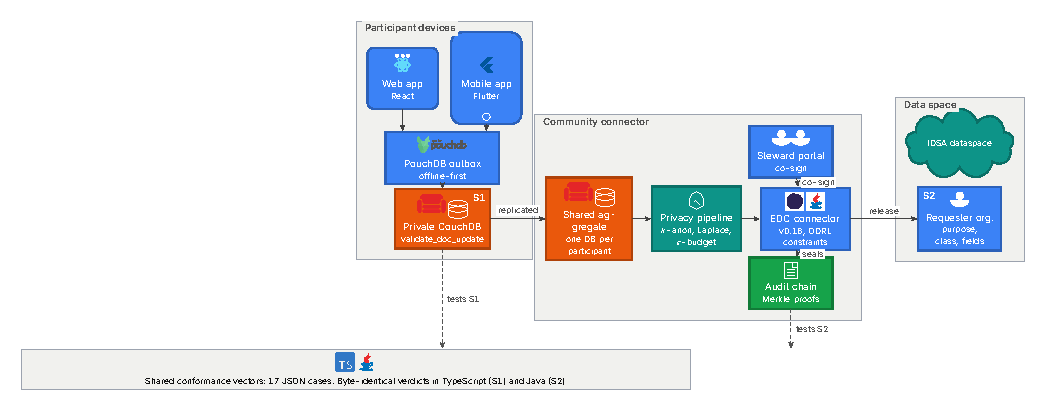
\includegraphics[width=\linewidth, totalheight=0.95\textheight, keepaspectratio]{../figures/schematics/fig-system-architecture.pdf}
\caption{The full system architecture, tier by tier, from participant devices through the community connector to the data space.}
\label{fig:architecture}
\end{figure}

\begin{figure}[H]
\centering
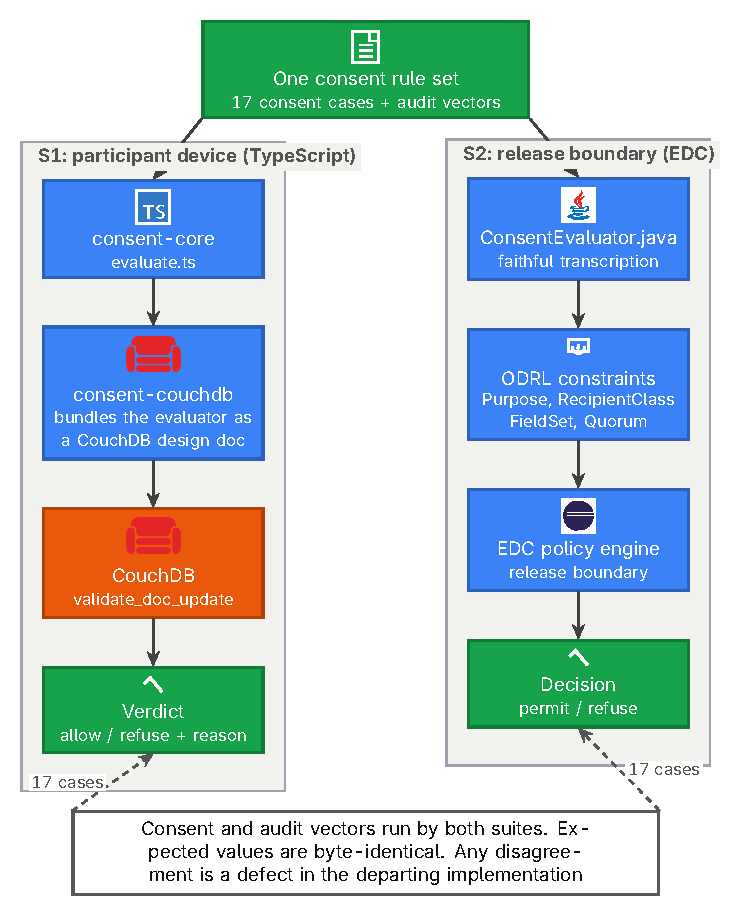
\includegraphics[width=\linewidth, totalheight=0.85\textheight, keepaspectratio]{../figures/schematics/fig-enforcement-points.pdf}
\caption{The two enforcement points, the CouchDB validator at the device boundary and the EDC constraint functions at the connector boundary, pinned together by the shared conformance vectors.}
\label{fig:enforcement-points}
\end{figure}

\begin{figure}[H]
\centering
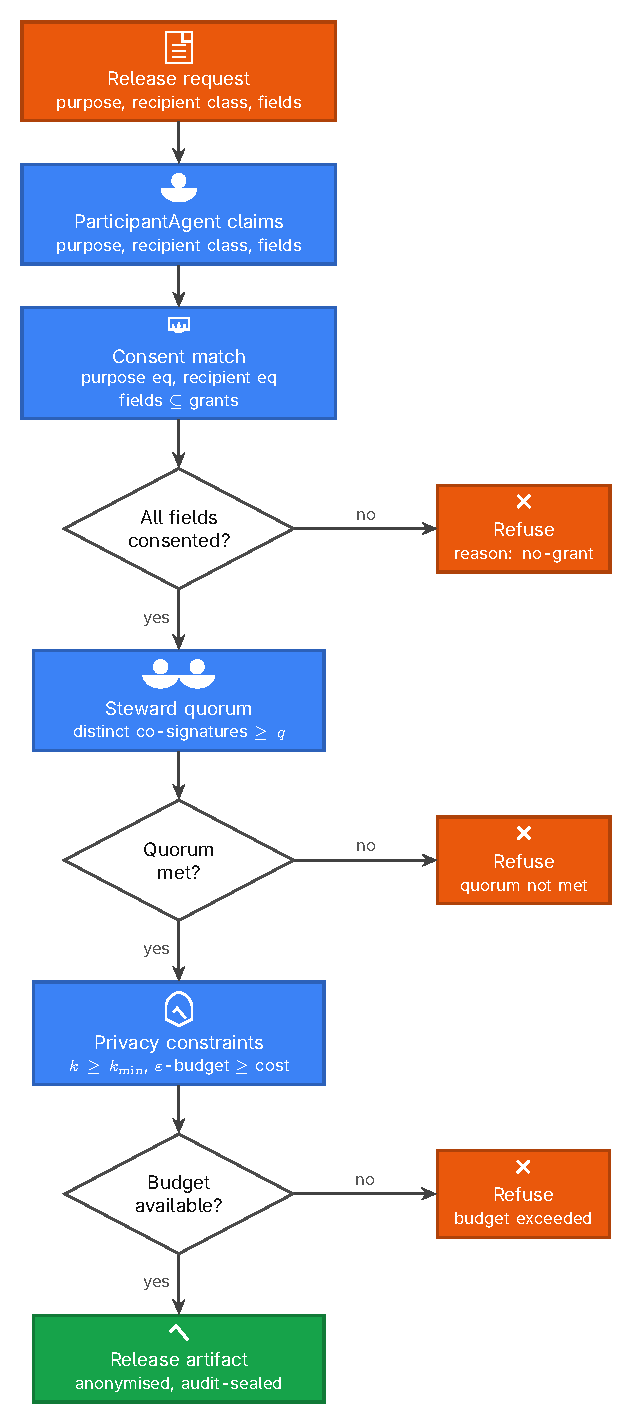
\includegraphics[height=0.85\textheight, keepaspectratio]{../figures/schematics/fig-release-flow.pdf}
\caption{The release decision flow, from request through consent checks to the steward quorum, privacy pipeline, and release.}
\label{fig:release-flow}
\end{figure}

\begin{figure}[H]
\centering
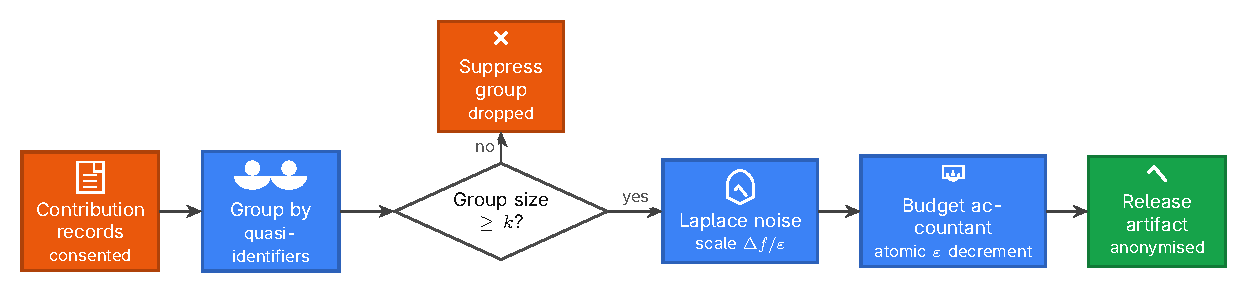
\includegraphics[width=\linewidth, totalheight=0.95\textheight, keepaspectratio]{../figures/schematics/fig-privacy-pipeline.pdf}
\caption{The privacy pipeline stages: records, grouping, k-anonymity, Laplace noise, and budget accounting.}
\label{fig:privacy-pipeline}
\end{figure}

\subsection{The EDC Connector Layer}

The design decision that shapes everything downstream is the choice to build the release boundary on a real IDSA-conformant connector rather than an application-level approximation of one. Eclipse Dataspace Components (EDC) provides the ODRL policy model, a policy engine with pluggable constraint functions, contract negotiation over the Dataspace Protocol, data plane and signaling infrastructure, and an event framework. It provides nothing for the offline-first device tier, the participant or steward interfaces, k-anonymity and differential privacy, or a participant-verifiable audit trail: those are the parts this project had to build itself, as the three connector extensions below and the TypeScript packages in section 3.3 describe.

EDC is pre-1.0 software with a roughly quarterly release cadence that has repeatedly shipped breaking changes. The reference implementation pins the connector to version 0.18.0 exactly and vendors the Gradle wrapper, recording the pin so that the manuscript's own reproducibility claims are attributable to a fixed dependency rather than a moving target. The 0.18.0 release alone changed the connector's default to data plane signaling, moved identity claims into the JWT \texttt{sub} claim, and replaced role-based authorization with scope-based authorization, any one of which would have silently invalidated an implementation written against the connector's documentation rather than its source. Identity in this deployment uses EDC's mock identity module (\texttt{org.eclipse.edc:iam-mock}) rather than IdentityHub with decentralized identifiers and verifiable credentials. Every claim this paper makes concerns what happens after a participant is already identified, so a full decentralized-identity stack was deliberately deferred rather than treated as a prerequisite, and this is stated here as a limitation rather than left implicit.

Registering a custom constraint function, binding it into the negotiation scope, and subscribing to connector events all had to be read from the 0.18.0 source directly rather than from documentation, because the release changed the shapes of exactly those APIs. Two further behaviors of the policy engine, discovered only by testing against a running connector rather than assumed from the design, are worth stating because they mark the implementation as real software rather than a paper design: EDC's management API rejects a policy definition outright, at creation time, if any of its constraints are bound to a scope but not to a registered function, so a compiler that emits a constraint ahead of the function that enforces it fails loudly rather than silently passing an unenforced rule. And the same API throws a \texttt{ClassCastException} on a numeric constraint right-operand, so the \texttt{consent-odrl} compiler in this implementation serializes every numeric threshold, including the steward-quorum count, as a string. Both are the kind of finding a specification cannot produce and only a build against the real connector can.

Three extensions realize the community-facing side of that connector. \texttt{benefits-policy} registers the BENEFITS-specific left operands the ODRL policy engine evaluates during contract negotiation, \texttt{PurposeFunction}, \texttt{RecipientClassFunction}, and \texttt{FieldSetFunction} for the consent-derived constraints, and \texttt{StewardQuorumFunction} for the release gate described in section 3.4. \texttt{benefits-privacy} implements the k-anonymity and differential-privacy pipeline described in section 3.5, exposed to the policy engine through its own \texttt{KAnonymityFunction} and \texttt{EpsilonBudgetFunction}. \texttt{benefits-audit} subscribes to the connector's event router and builds the Merkle-epoch audit chain described in section 3.6. This is a consolidation of the original design's four planned extensions, \texttt{benefits-policy}, \texttt{steward-quorum}, \texttt{privacy-pipeline}, and \texttt{audit-chain}, into three: the steward-quorum constraint function and its supporting store live inside \texttt{benefits-policy} alongside the other consent-derived constraint functions, rather than in a fourth, separate module.

Positioning this deployment against the closest comparators identified in the literature search is instructive about what "EDC in production" currently looks like elsewhere. \cite{mugge2023} implement a Catena-X connector, built on the same EDC family, for cross-company end-of-life-vehicle decision support, and validate it against a real cross-company data flow between named industrial roles. It is the strongest existing evidence that an EDC-based connector deployment can carry real, sovereignty-respecting data exchange for a concrete downstream use case rather than a synthetic demonstration, and this project's own community-connector deployment sits in the same thin but active empirical space. \cite{kalogeropoulos2023} integrate an IDS-connector-as-a-service into a Multi-access Edge Computing architecture and report scalability experiments, one of the few sources in this space with any quantitative evaluation, though at the edge-computing layer rather than at the connector's own policy-enforcement layer. \cite{norikane2025}, published in this paper's own target venue, model a data-space-based manufacturing supply chain and simulate its resilience under disruption. It evaluates supply-chain outcomes rather than connector-level properties, but it establishes that MDPI Systems already publishes verified, technically evaluated work on built data-space deployments, which is the venue precedent this chapter's own connector description follows.

\subsection{Paying for the Two-Language Boundary}

The choice to build the release boundary on a real connector has a direct cost: the connector is Java, and the device-tier consent filter has to run inside CouchDB's JavaScript validation engine, so the same consent semantics exist in two languages with no shared runtime between them. A single-language monorepo, considered and rejected during design, could have claimed one implementation of consent semantics shared by every enforcement point. The connector-based approach cannot make that claim, because the S1 evaluator at the device boundary and the S2 constraint functions at the connector boundary are necessarily separate code, written in separate languages, and free to drift apart without anyone noticing.

The consent model itself is designed once and compiled twice. \texttt{packages/consent-core} defines the rule model as a per-field grant of \texttt{(field, purpose, recipient class)}, its meet-semilattice composition operation (\texttt{meet.ts}, used when a released dataset draws on many participants whose grants differ, taking the narrowest purpose set, narrowest recipient class, intersection of fields, and earliest expiry across all of them), and the S1 evaluator itself (\texttt{evaluate.ts}). Two packages compile that single model into the system's two enforcement points: \texttt{consent-couchdb} bundles it into the CouchDB design document that becomes the \texttt{validate\_doc\_update} function running server-side inside CouchDB's own sealed query-server engine, and \texttt{consent-odrl} compiles it into the ODRL JSON-LD policy document that EDC's contract negotiation evaluates through the \texttt{benefits-policy} extension's constraint functions. TypeScript and Java exchange nothing but that JSON policy document. There is no shared library, shared type definitions, or remote procedure call between the two enforcement points, only an artifact both sides independently interpret.

That gap between two independent interpretations of the same document is exactly where drift becomes possible, and it is the one place in this design where a genuine engineering risk was accepted rather than designed away. The mitigation is a shared conformance-vector suite: a set of JSON test cases, each describing one grant configuration and one attempted access, that both the CouchDB validator and the connector's constraint functions must decide identically. The repository carries seventeen such vectors (\texttt{conformance/vectors}, covering cases such as a simple allowed access, a missing grant, an expired grant, a participant mismatch, and a purpose mismatch), each run against both implementations in their respective test suites, \texttt{ConformanceVectorTest} on the Java side and the corresponding suite in \texttt{consent-couchdb}'s own tests on the TypeScript side. The audit chain applies the identical strategy for its own two-sided risk, hashing computed on the connector side and re-verified on the participant side, with six further vectors (\texttt{conformance/audit-vectors}) exercised by \texttt{AuditConformanceVectorTest}. Table 1 lists all twenty-three vectors, the seventeen consent cases and the six audit cases, with the specific case each one exercises.

\begin{table}[H]
\caption{Consent and audit conformance vectors, with the specific case each one exercises.\label{tab:t1}}
\begin{tabularx}{\textwidth}{llX}
\toprule
Suite & Vector ID & What it tests \\
\midrule
Consent & v001-simple-allow & one field with an exactly matching unexpired grant \\
Consent & v002-missing-grant & a second field is present with no grant covering it \\
Consent & v003-expired-grant & the only grant for the field expired before now \\
Consent & v004-participant-mismatch & \texttt{consent.participantRef} differs from \texttt{record.participantRef} \\
Consent & v005-purpose-mismatch & \texttt{declaredPurpose} does not match the grant's purpose \\
Consent & v006-recipient-class-mismatch & \texttt{declaredRecipientClass} does not match the grant's recipient class \\
Consent & v007-not-a-contribution & type is not \texttt{contribution}, so S1 does not apply \\
Consent & v008-missing-consent & the \texttt{consent} property is absent from the record \\
Consent & v009-multi-field-ordering & several fields lack a covering grant. The alphabetically first one is reported \\
Consent & v010-expiry-exact-instant & a grant whose \texttt{expiresAt} equals now is expired (exclusive boundary) \\
Consent & v011-granted-at-exact-instant & a grant whose \texttt{grantedAt} equals now is active (inclusive boundary) \\
Consent & v012-null-grants & a \texttt{grants} value of null is treated as a missing consent assertion \\
Consent & v013-empty-grants & an empty \texttt{grants} array is present but grants nothing, so an uncovered field is reported \\
Consent & v014-malformed-fields & \texttt{fields} is a JSON array rather than the contracted object \\
Consent & v015-empty-string-grants & \texttt{consent.grants} is an empty string, neither absent nor null \\
Consent & v016-revoked-grant & a grant revoked before the record's evaluation instant is inactive \\
Consent & v017-revocation-not-yet-effective & a revocation timestamped after the evaluation instant has not taken effect yet \\
Audit & av001-single-leaf & a single-entry tree. The root is that entry's own leaf hash \\
Audit & av002-two-leaves & an even-sized tree, one pairing, no promotion \\
Audit & av003-three-leaves-odd-promotion & an odd-sized tree. The third leaf is promoted unhashed to the second level \\
Audit & av004-five-leaves & a larger odd-sized tree spanning two levels of promotion \\
Audit & av005-separator-in-plain-language & a field value containing the raw separator character, escaped identically in both languages \\
Audit & av006-backslash-in-actor & a field value containing a raw backslash, escaped identically in both languages \\
\bottomrule
\end{tabularx}
\end{table}

This converts a structural weakness into a publishable artifact rather than merely patching around it. As the design record for this project puts it, releasing a set of conformance vectors and demonstrating that edge and connector enforcement agree on all of them is a stronger correctness claim than asserting the code was written once, because the claim survives exactly the failure mode a single shared implementation cannot even expose: two independent implementations reaching the same decision on every case that matters, not by construction, but by test.

Both of the enforcement points just described, the S1 evaluator at the device boundary and the S2 constraint functions at the connector boundary, gate writes: whether a record may leave the device and whether a release may be negotiated. Neither, as originally built, gated whether an already-written contribution could be included in a query-time aggregate: \texttt{Contribution}, the record type \texttt{benefits-privacy}'s \texttt{PrivacyPipeline} and \texttt{KAnonymity} actually operate on, carried no consent information at all, so an aggregate query result could include a contribution regardless of the consent scope its owner had actually granted, once that contribution had already been written. This gap went unaddressed until the G2 experiment (Chapter 5, Chapter 6) required closing it. Doing so meant building query-time consent scoping into \texttt{PrivacyPipeline} itself, wiring a new \texttt{ConsentGrant} type and a query-purpose-and-recipient-class filter into the production pipeline rather than into the experiment harness alone, so this is a real, additive production capability this project added, not a test fixture confined to G2.

\subsection{The Steward-Quorum Release Gate}

SIDS 2026's own description of the steward gate was explicit and specific: aggregated outputs wrapped in a cryptographic envelope keyed by steward quorum, with the decryption key released only on receipt of a co-signed authorization token, and the reference-implementation design that followed it retained Shamir secret sharing over the payload content key as, in its own framing, a second lock on release, because a policy engine the operator runs is not the same guarantee as cryptographic impossibility, and that difference is exactly what a skeptical reviewer would press on.

That cryptographic second lock was not carried into the built system. The \texttt{benefits-policy} extension's \texttt{StewardAuthorization} record holds a release request identifier, a dataset hash binding the token to an exact dataset, a list of steward signatures, and separate lists of reviews, vetoes, and appeals. It carries no key shares, and no component of \texttt{benefits-privacy}'s \texttt{ReleaseArtifact} store encrypts its bytes under a quorum-reconstructed key. What is actually enforced is a signature-count threshold: \texttt{StewardQuorumFunction}, registered as an ODRL constraint function and evaluated during contract negotiation, reads the release request identifier from a sibling constraint on the same permission (EDC's policy context carries no general-purpose data map, so the quorum function locates its state this way rather than off the evaluation context directly), looks up the corresponding \texttt{StewardAuthorization}, counts the number of distinct stewards who have signed it, and refuses the negotiation unless that count meets or exceeds the threshold the policy names. Contract negotiation cannot complete without that quorum, so the gate is real and release-blocking, but the mechanism realizing it is a policy-engine check against a database-backed authorization record, not a cryptographic envelope that makes unauthorized release mathematically impossible regardless of who operates the connector. This is a narrower guarantee than SIDS 2026 described and than the design specification that followed it originally called for, and the manuscript states that gap here rather than silently rewriting the earlier claim to match what was built.

A second gap, more serious than the cryptographic one just stated, sits alongside it. SIDS 2026's own text specifies a veto, not merely a quorum, as part of the steward gate: "for each release, two of three rotating stewards must co-sign an authorization token; any single steward may veto, in which case the release request is returned to the requester with a written justification" \cite{katrakazas2026}. The built system does not enforce this. \texttt{StewardQuorumFunction.evaluate} reads only \texttt{authorization.distinctStewardCount() >= required}. It never reads \texttt{authorization.vetoes()}, confirmed directly in the source. A steward can record a veto today, through the same \texttt{StewardAuthorization} record that already carries a \texttt{vetoes} list alongside its signatures, reviews, and appeals, but that recorded veto has no effect on whether contract negotiation succeeds: a release with a satisfied signature count clears the gate whether or not a steward has vetoed it. It is the predecessor paper's own specified policy, published before this system was built, and the built system silently does not enforce it. Unlike the cryptographic-envelope gap, which diverges from an internal design intent that a reference implementation stopped short of realizing, this gap diverges from a guarantee SIDS 2026 explicitly promised its readers, which is why it is treated here as the more serious of the two.

That gap changes how this mechanism should be read against its closest technical comparators. \cite{kokoriskogias2020} describe CALYPSO, in which confidential "on-chain secrets" require an actual threshold of a trustee committee to decrypt, benchmarked directly against committee size, with latency scaling from roughly 0.2 to 8 seconds as the committee grows from 16 to 128 members. Release there is gated by genuine threshold decryption, so no subset of the committee smaller than the threshold can produce the plaintext under any circumstance. \cite{raisaro2019} describe MedCo, a deployed clinical and genomic data-sharing system in which decrypting pooled query results requires the collective participation of every federated site holding a key share, again a real distributed-decryption gate rather than a policy check. Both are stronger comparators in the cryptographic sense than a contrast: they hold the property the original BENEFITS design aspired to and the built system does not yet realize. What this implementation does hold in common with them is the auditable, quorum-of-independent-parties structure around the release decision: signature, review, veto, and appeal records are all held alongside one another in \texttt{StewardAuthorization}, and the framing that a single actor should never unilaterally control disclosure. What it does not yet hold is CALYPSO's and MedCo's cryptographic independence from the operator of the software making the check, and, per the veto gap stated above, the recorded vetoes it does hold are not yet consulted by the release decision itself. A veto is recorded, not enforced. Stating this precisely, rather than describing the built gate as equivalent to threshold decryption, is itself part of what this chapter reports about the system as it currently stands.

\subsection{The Privacy Pipeline}

The \texttt{benefits-privacy} extension implements the anonymization stage SIDS 2026 described as an architectural primitive rather than a compliance afterthought. \texttt{KAnonymity} computes the structural k of a candidate release and \texttt{KAnonymityFunction} exposes that computation to the policy engine as an ODRL constraint, so a release whose computed k falls below the policy's threshold is refused at contract negotiation rather than filtered after the fact. \texttt{LaplaceNoiseSource}, sitting behind the shared \texttt{NoiseSource} interface, adds calibrated Laplace noise to statistical query results, and \texttt{BudgetAccountant} (with \texttt{InMemoryBudgetAccountant} and \texttt{CouchDbBudgetAccountant} implementations) tracks cumulative privacy loss against a per-site budget, exposed to the policy engine through \texttt{EpsilonBudgetFunction} so that a query exceeding the remaining allowance is refused the same way an under-threshold k value is. \texttt{PrivacyPipeline} composes k-anonymity, noise addition, and budget accounting into the sequence a release request actually passes through, and \texttt{ReleaseArtifact} stores the computed result once rather than recomputing it per transfer, a deliberate choice: recomputing per transfer would let a requester repeat the same transfer and average results to recover the true value while the budget accountant had charged epsilon only once, defeating the accounting it exists to enforce.

Two of these constraint functions did not exist when the connector's policy compiler was first written, and the design specification is explicit that this was tested against a running connector rather than assumed: EDC rejects an entire policy document at creation time if it names a constraint bound to no registered function, so \texttt{consent-odrl} could not emit \texttt{benefits:kAnonymity} or \texttt{benefits:epsilonBudget} constraints until \texttt{KAnonymityFunction} and \texttt{EpsilonBudgetFunction} existed to enforce them, and the compiler's options for those two constraints were removed from its interface entirely in the interim rather than left present but silently unenforced, on the reasoning that an option a caller can set while nothing checks it is a false affordance worse than no option at all.

This pipeline sits between two identifiable lines of prior work. \cite{mironov2017} supplies the theoretical grounding much of the modern budget-accounting literature is built on, Rényi differential privacy, a relaxation that generalizes and recovers the moments-accountant approach as a special case and admits substantially tighter composition than naive sequential composition, and the accounting discipline behind \texttt{BudgetAccountant}'s cumulative-loss tracking descends from that same lineage even though the pipeline itself uses simple Laplace mechanisms rather than an RDP-based accountant specifically. \cite{prasser2020} describe ARX, an actively maintained, real anonymization tool that combines k-anonymity and related structural models with a differential-privacy mode and built-in utility metrics, the closest existing tool that pairs structural anonymization and formal DP the way this pipeline's \texttt{KAnonymity} stage and \texttt{LaplaceNoiseSource} stage are paired here. Where ARX is a general-purpose, standalone anonymization tool applied after the fact to a dataset, \texttt{benefits-privacy}'s pipeline is embedded directly in the connector's contract-negotiation path, so a release that would violate either bound is refused before data leaves the boundary rather than flagged by a separate tool a step later.

\subsection{The Audit Chain}

\texttt{benefits-audit} implements the tamper-evident record SIDS 2026 described as hash-chained, but batches entries into epochs rather than chaining every entry directly, on a specific design rationale: a pure hash chain forces a verifying participant to hold every entry in the log to check their own, which leaks the existence and timing of other participants' access events to anyone checking their own record. Instead, \texttt{MerkleTree} builds a Merkle tree over the entries within one epoch, \texttt{EpochSealer} seals that epoch by committing its root, and \texttt{AuditHashing} chains only the epoch roots to one another, so a participant can obtain their own entries, an inclusion proof for each, and the root chain, proving their entries are present and unaltered while learning nothing about anyone else's. \texttt{BenefitsAuditEventListener} subscribes to the connector's \texttt{EventRouter} and is the component intended to make the log a record of what the connector actually did rather than something an application component writes about itself. \texttt{AuditStore}, with \texttt{InMemoryAuditStore} and \texttt{CouchDbAuditStore} implementations, persists the resulting entries and epochs, and the paired TypeScript package \texttt{audit-verify} (\texttt{chain.ts}, \texttt{hashing.ts}, \texttt{merkle.ts}) implements the participant-side half of the same verification, so that inclusion and consistency checks do not depend on trusting the connector that produced them.

The claim that the log records "every negotiation, policy decision, and transfer" was written before any EDC event had ever been observed firing, and testing it against a running connector overturned part of it. A negotiation offer refused because it fails ODRL constraint evaluation, whether for missing steward quorum, purpose mismatch, recipient-class mismatch, an out-of-grant field, an expired grant, insufficient k, or an exhausted privacy budget, is rejected by EDC 0.18.0 synchronously, inside its Dataspace Protocol handler, before any \texttt{ContractNegotiation} entity is created. Because EDC's event system fires only from state-machine transitions on entities that exist, and no entity is created for this class of refusal, no event is ever published for it. This was confirmed empirically by forcing a real policy-refused negotiation against a running provider and observing a 400 response paired with zero corresponding lines in the provider's own event log. The audit chain therefore does not cover the conformance suite's refusal cases specifically, precisely the "policy decision" the steward-quorum, k-anonymity, and epsilon-budget machinery exists to make. What it does cover is every negotiation admitted into the provider's state machine, whether it later succeeds or is terminated, and every transfer attempt. A cheaper fix, having a constraint function record its own refusal into the log the moment it returns false, was considered and rejected, because it would restore coverage only by having the log contain entries an application component chose to self-report, exactly where independent, connector-native proof matters most. This boundary, not the original "every policy decision" phrasing, is what this paper claims about the audit chain's coverage.

Positioned against prior art, the mechanism descends directly from \cite{schneier1999}, whose scheme couples chained one-way hashes, which establish the retroactive-tamper-detection guarantee that any alteration of an already-hashed entry breaks the chain from that point forward, with forward-secure MACs, which are what make entries written before a compromise unreadable to an attacker who later controls the logging machine. SIDS 2026's own architecture section invokes the tamper-detection half of this guarantee without tracing it to a source. The epoch structure itself follows the real-world deployed precedent of Certificate Transparency \cite{laurie2013}, which defines standardized Merkle audit paths and consistency proofs for publicly logging TLS certificate issuance and has run at internet scale since its 2013 publication as RFC 6962, later superseded by RFC 9162 (Certificate Transparency Version 2.0). Major browsers required Certificate Transparency for TLS certificates for several years following its deployment. Where Certificate Transparency's epochs are global and its proofs are about certificate issuance visible to any observer, this system's epochs are sealed periodically over participant contribution events and its inclusion proofs are scoped so a participant learns only about their own entries, the privacy property the pure hash-chain alternative could not offer.

\subsection{What the Phase Gates Verified}

The build proceeded through eight gated phases, each required to pass before the next began, because the correctness claims in this design are the contribution and needed to be test-first rather than retrofitted. What the gates actually established, rather than what was merely planned, is the honest summary of what this chapter can claim as built. The skeleton phase established that the pinned connector's Management API answers, that CouchDB is reachable, and that a custom constraint function can be observed evaluating during a real two-connector negotiation, with the CouchDB query server's engine probed and recorded rather than assumed. The consent-core phase established that the conformance vectors pass and that a real CouchDB instance, running the compiled validation function, rejects an unconsented write. The policy and steward-quorum phase established that the consent-derived conformance cases pass and that contract negotiation is refused without a satisfied steward quorum, against a running connector rather than a mock. Table 2 lists all nine cases this phase's gate checked, each a real contract negotiation against the connector rather than a unit test. All nine passed.

\begin{table}[H]
\caption{Enforcement-correctness cases checked at the policy and steward-quorum gate. All nine passed.\label{tab:t2}}
\begin{tabularx}{\textwidth}{lllX}
\toprule
Case & Expected & Observed & Discriminating evidence \\
\midrule
quorum-met & FINALIZED & FINALIZED & signed=2, required=2 \\
quorum-missing & TERMINATED & TERMINATED & no steward authorization seeded for the request \\
quorum-one-steward-twice & TERMINATED & TERMINATED & two signatures from one steward counted as signed=1 \\
purpose-mismatch & TERMINATED & TERMINATED & requester purpose \texttt{marketing} against policy purpose \texttt{service-improvement} \\
recipient-class-mismatch & TERMINATED & TERMINATED & requester recipient class \texttt{provider} against policy \texttt{statistics} \\
field-outside-grant & TERMINATED & TERMINATED & requested \texttt{health.condition} outside granted \texttt{service.satisfaction} \\
expired-grant-field-excluded & TERMINATED & TERMINATED & expired \texttt{health.condition} grant excluded from the compiled policy \\
k-below-threshold* & TERMINATED & TERMINATED & \texttt{computedK}=4 below \texttt{required}=5 \\
budget-exceeded* & TERMINATED & TERMINATED & \texttt{charged}=0.9 above \texttt{cap}=0.5 \\
\bottomrule
\end{tabularx}
\end{table}

The two cases marked with an asterisk exercise \texttt{KAnonymityFunction} and \texttt{EpsilonBudgetFunction} against a directly-seeded \texttt{ReleaseArtifact} rather than one produced by a live \texttt{PrivacyPipeline} run. The artifact's \texttt{computedK} and \texttt{epsilonCharged} are seeded values chosen to land on each side of the policy threshold, not values the pipeline itself computed from real contributions. \texttt{PrivacyPipeline.compute} is proven separately, end to end, by \texttt{PrivacyPipelineTest}, \texttt{KAnonymityTest}, \texttt{LaplaceNoiseSourceTest}, and \texttt{InMemoryBudgetAccountantTest}.

The audit-chain phase established that mutated entries, mutated roots, and reordered epochs are each detected at the mechanism level in every case tested, with the formal proof-size and verification-time sweep against epoch size deferred to the later experiment phase rather than folded into this gate. The device-fleet phase and the interface phase built the simulated PouchDB fleet used for the revocation-under-partition experiment and manually click-tested the participant-web and steward-portal applications, producing the screenshots this manuscript can draw on. That fleet's revocation mechanism is a client-side purge, not a server-side re-check: \texttt{Device.revoke} mutates the device's own local grant state and, in the same call, removes any not-yet-synced contribution record matching the revoked field, purpose, and recipient class from the device's local queue, before that record is ever replicated to CouchDB. The CouchDB \texttt{validate\_doc\_update} function does not provide an independent second check of this: it evaluates a contribution record's own embedded \texttt{consent.grants} snapshot, taken at write time, against the live server clock, but it has no access to the device's current grant state and so cannot detect that a grant embedded in an already-queued record has since been revoked. A queued record the device failed to purge before syncing would still pass that validation on its stale, embedded consent. E2's zero-leaked-record result (section 5.2) therefore verifies that the device-side purge works on every tested duty cycle, not that the server independently catches what the device failed to withhold.

Taken together, these gates are the evidentiary basis for the claim this chapter opened with: the architecture SIDS 2026 sketched is now real, running software, not a specification awaiting pilot deployment. That software is not identical to the design that preceded it. The steward-release gate is a policy-engine check backed by a signature quorum rather than the cryptographic envelope originally proposed, that same gate does not enforce the single-steward veto SIDS 2026 specified even though it records vetoes, and the audit chain's coverage stops at the boundary of policy-refused negotiations rather than extending to every policy decision as first written. Reporting all three corrections plainly, alongside what the gates did establish, is what distinguishes this chapter's account of the system from the specification it replaces.

\section{Experimental Methodology}

The System Architecture chapter established that BENEFITS is a running system, not a specification: the EDC connector extensions, the consent packages, and the audit and privacy pipelines all execute against real infrastructure and pass a two-language conformance-vector suite, C1, that proves the TypeScript edge-side evaluator and the Java connector-side evaluator agree on every conformance case. C1 is a correctness baseline, not a performance or robustness claim: it establishes that consent is evaluated identically wherever it is evaluated, but it says nothing about what that evaluation costs, how the architecture behaves when its assumptions are stressed, or where its guarantees degrade under realistic operating conditions. Six mechanism-level experiments build on that baseline to answer exactly those questions. Each experiment targets one open question the architecture's design left unsettled at specification time, each is driven by a seeded, deterministic harness whose full parameter grid and repeated trials produce reproducible results from a committed seed, and each writes its output to a committed CSV under \texttt{experiments/results/}, so every number reported in Chapter 5 traces back to a specific, rerunnable sweep rather than a one-off measurement. This chapter describes what each experiment measures, how its parameter space is swept, and what statistics are computed over the results. It does not report or characterize the results themselves, which are reserved for Chapter 5.

\subsection{E1: Signature-Verification Cost at the Edge}

The architecture's participant-side enforcement (S1) is a \texttt{validate\_doc\_update} function installed on each participant's own CouchDB database, evaluated inside CouchDB's own JavaScript query-server engine rather than on-device. SIDS 2026 left open whether this design could be extended with cryptographic assurance, specifically whether a pure-JavaScript Ed25519 signature verification routine, running inside that same constrained query-server engine, is fast enough to be viable at any realistic batch size or fails outright. E1 answers this by measuring real HTTP writes against a real CouchDB instance under three arms: a baseline with no validator installed (isolating CouchDB's own request and storage overhead), the existing structural validator unchanged, and a third, experiment-only design document that performs the same structural check and additionally verifies an Ed25519 signature over each record. The signature-verifying arm exists only inside the experiment harness. It is never installed by any production provisioning path.

Each arm is swept across three dimensions: batch size (10, 50, 100, 500, 1000, 5000, 10000 documents, log-spaced), field count per record (1, 5, 20), and grant-set size (0, 10, or 50 decoy grants added ahead of each field's real grant, chosen specifically because consent-core's grant lookup scans linearly and returns on first match, so decoy count, not field count, is what determines how far that scan actually has to walk). The full cross product is 63 configurations per arm, each repeated across 3 trials to give the results a basis for reporting variance rather than a single point per cell, run against a throttled container fixed at one CPU core and 1 GB of memory to approximate the class of low-end handset the target population is expected to own, with the host CPU model recorded alongside every row so the throttle quota is interpretable rather than assumed reproducible across machines. Wall-clock time is measured client-side around each write batch.

\subsection{E2: Revocation Propagation Under Network Partition}

The device-fleet phase of the reference implementation already proved, at the mechanism level, that a participant who revokes consent while offline with records already queued produces zero leaked records once connectivity resumes, and that conflicting concurrent writes converge under the project's "user preference first" resolution strategy. E2 is the formal, swept version of that same mechanism: it asks how revocation propagation latency and time-to-consistency vary with connectivity, not merely whether the guarantee holds at one hand-built connectivity pattern.

The experiment simulates a fleet of 10 devices per trial, split into three fixed roles: three revocation devices, each of which queues an ordinary record and then revokes consent for it while still offline, before any sync has occurred. Three conflict devices, each of which writes a document under a known identifier and then has a rival remote revision injected against it. And four baseline devices that contribute ordinary records with no revocation or conflict, giving the trial's leaked-record and consistency checks real successful writes to check against. Each device runs its own duty cycle governing when it comes online, and the one swept dimension is that duty cycle's online probability: 0.05, 0.1, 0.3, 0.5, and 0.9, spanning near-permanent offline to near-permanent online. Thirty independent fleet trials run at each of the five sweep points, for 150 trials in total, each trial running for up to 200 simulated ticks. After each device completes its tracked action, the harness checks the shared CouchDB database directly for any leaked record matching a revoked participant and purpose, and checks that every conflict document's conflict list has been fully resolved. Either check failing increments a defect counter rather than being folded into a graceful statistic. For the timing behavior, the harness records the median and interquartile range of propagation ticks (for revocation devices) and consistency ticks (for conflict devices) pooled across all 90 data points collected per sweep point, alongside the leaked-record and unresolved-conflict counts, which the design treats as pass/fail correctness gates rather than as distributions to characterize.

\subsection{E3: Audit-Chain Verification Cost at Scale}

The audit-chain mechanism's boolean correctness, that a mutated leaf, root, or proof step fails verification, and that a reordered or altered epoch is caught by chain verification, was already proven at the unit level during an earlier implementation phase. What that phase deliberately deferred was the question SIDS 2026 left open: epoch length trades proof size against sealing latency, and the reference implementation needed to know what that tradeoff actually costs on the participant's own device as the audit structure scales. E3 supplies that measurement without touching the correctness logic itself. It adds timing and size instrumentation around calls that already exist.

Two dimensions are swept. Epoch size (10, 50, 100, 500, 1000, 5000 entries, log-spaced) governs proof size and inclusion-proof verification time: for each epoch size, the harness builds one Merkle tree and samples inclusion proofs at 10 evenly spaced leaf positions (or every leaf, below 10), recording the number of proof steps and the resulting proof size in digest bytes. Because a single inclusion-proof verification is sub-millisecond even at the largest epoch size, each fixture is timed across 10 repetitions after an untimed warmup pass, and the median of those repetitions is recorded, following the same repeated-trial convention E1 uses to make a sub-millisecond measurement reportable at all. Chain length (5, 20, 100, 500 epochs) governs chain verification time separately, since verifying the chain only recomputes and compares epoch-to-epoch hash links and its cost does not depend on epoch size at all. Sweeping it against epoch size would produce no informational content, so it is measured against chain length instead, using the same warmup-then-median-of-ten-repetitions protocol. All fixture generation is seeded so results reproduce from a committed seed, and inclusion-proof verification runs under the same throttled, low-end device profile as E1, since that is the code path a participant's own device actually executes. This experiment follows most directly from \cite{crosby2009}, who established proof size and verification cost as the metric of interest for tree-structured tamper-evident logs and measured both as a function of log scale, and it sits alongside \cite{melara2015} and \cite{hu2021}, whose Merkle-based transparency logs report comparable proof-size- and latency-versus-scale curves under their own scale parameters. E3 departs from all three by sweeping epoch size specifically rather than overall log or user-base scale, since epoch size is the parameter this architecture's own sealing design exposes as a tunable tradeoff.

\subsection{E4: Privacy-Budget-Versus-Utility Tradeoff}

SIDS 2026 raised, as an open governance challenge rather than a settled design, the concern that differential privacy could render aggregate statistics analytically meaningless at the population scale of an individual service site. E4 answers this directly by driving the privacy pipeline's existing, unmodified k-anonymity, Laplace-noise, and budget-accountant classes with synthetic query workloads and measuring accuracy as a function of privacy budget, population size, and the k-anonymity threshold, rather than modifying any of the production classes under test.

A seeded population generator produces synthetic contributions with three quasi-identifier attributes (service type, channel, urgency level), under two distribution modes: uniform, and a skewed mode in which channel preference is fixed at 61 percent paper contact, matching the one workshop statistic from the parent study that maps directly onto a swept attribute. The remaining attribute skews are declared assumptions rather than workshop-sourced figures, stated as such. Eight queries are run per sweep point in a fixed order against one shared budget accountant per synthetic site: three grouped counts (over service type, channel, and urgency level, chosen for their differing category cardinalities), two proportions (the largest service-type group's share, and a fixed rare category's share), and three cross-tabulations of increasing granularity. Running all eight against one shared accountant, rather than giving each query its own fresh budget, is deliberate: it is the only way to exercise the accountant's real, atomic, shared-budget behavior, which is exactly the property under test.

The sweep varies epsilon (the per-query privacy parameter: 0.1, 0.27, 0.31, 0.37, 0.5, 1.0, 1.5, and 2.0, with the three added values chosen specifically to fall inside the epsilon range where the number of queries a fixed total per-site budget of 2.0 can still afford actually changes, since a coarser five-point grid was found to sit entirely on one side of that transition and produce a degenerate result), site population (30, 100, 200, 300), and the k-anonymity threshold (3, 5, 7, 10), crossed with the two population-skew modes, for 256 total sweep points. Because the computation is deterministic given a seed, with no wall-clock variability to average out, each point runs once rather than across repeated trials. The median and interquartile range the parent design calls for are instead computed across the pooled per-group relative-error values the eight-query workload produces at that point. Three statistics are reported per point: the median and interquartile range of relative error across the full pooled set, with a fixed sentinel value of 1.0 assigned to any group that was suppressed by k-anonymity or any query refused for exhausted budget. The suppression/refusal rate itself, isolating how much of the workload received no answer at all. And a surviving-only median and interquartile range computed over only the subset of data points that were neither suppressed nor refused, isolating the accuracy of the answers that were actually returned from how often an answer was returned at all. This experimental shape, accuracy characterized as a function of privacy budget under a shared, enforced accountant, follows the precedent set by \cite{abadi2016}, who report the accuracy cost of a tracked privacy budget directly, and \cite{hay2016}, whose DPBench methodology establishes accuracy-versus-epsilon curves under a shared benchmark protocol as the standard empirical framing for this class of evaluation. \cite{rogers2021} supplies the closest production analogue, a deployed budget-management service enforcing a strict, shared differential-privacy budget on live queries at scale, structurally the same kind of accountant this experiment measures at a much smaller, per-site scale.

\subsection{G1: Quorum Availability Under the Built Policy and the Veto Policy SIDS 2026 Specified}

The steward-quorum mechanism requires a threshold number of stewards to co-sign before a data release proceeds. The built system's production decision function reads only the count of signing stewards. It never consults recorded vetoes, even though SIDS 2026's own text specifies a veto as part of the release gate, not merely a quorum: "any single steward may veto, in which case the release request is returned to the requester with a written justification" \cite{katrakazas2026}. G1 exists to answer what that gap leaves open: what does enforcing the veto guarantee SIDS 2026 specified, and the built system currently does not provide, cost in release availability as stewards go offline, act slowly, or object.

Two arms run on an identical, shared simulated timeline of steward actions. Arm A calls the real, unmodified quorum-decision class directly against a real, unmodified steward-authorization store as the timeline unfolds, the built system's own veto-blind policy. Arm B is a second decision function that exists only inside the experiment harness, explicitly documented as non-production, which adds exactly the check SIDS 2026 specified and the built system omits: a permanent block the moment any single steward vetoes. At each discrete tick, every steward who has not yet acted may act with a fixed per-tick probability, and, conditional on acting, may sign or veto according to a fixed veto share. A run terminates when both arms reach a determinate outcome, quorum reached for Arm A, quorum reached, permanently vetoed, or starved for Arm B, or at a 200-tick horizon chosen so that even the least favorable swept parameters leave the probability of an undetermined outcome negligible.

The sweep spans steward pool size (5, 10, 20), quorum size expressed as a fraction of the pool (0.3, 0.5, 0.7), per-tick action probability (0.1, 0.3, 0.5, 0.7, 0.9), and veto share among acting stewards (0.0, 0.1, 0.3, with 0.0 serving as a sanity check where Arm B degenerates to Arm A's own behavior), for 135 sweep points, each run across 200 independent seeded repetitions to characterize the distribution of a stochastic per-tick process rather than a single deterministic run. Per point, the harness reports each arm's reached rate, and, for Arm A, its starved rate, for Arm B, its reached, vetoed, and starved rates, which are mutually exclusive and sum to one, so that Arm B's failures can be decomposed into how much comes from vetoes actually landing versus genuine starvation rather than reported as one undifferentiated failure rate. Time-to-quorum is reported as the median and interquartile range of ticks, computed only over the runs that actually reached quorum in that arm, following the same surviving-only convention E4 established for its own accuracy statistic, so that an arm's speed and its reliability are reported as separate, uncombined statistics. This design mirrors the quorum-size-versus-performance evaluation shape established by \cite{kokoriskogias2020}, whose CALYPSO system measures transaction latency as trustee-committee size scales, the closest direct precedent in the literature for characterizing a threshold-committee's behavior as a tunable tradeoff between committee size and system outcome, here reliability rather than latency, under a two-arm comparison between the built, veto-blind policy and the veto-enforcing policy SIDS 2026's own text specifies.

\subsection{G2: Consent Heterogeneity Versus Aggregate Utility}

The architecture's consent model gates writes but, before this experiment, gated nothing at query time: an already-written contribution had no mechanism preventing its inclusion in an aggregate query result regardless of what purposes or recipient classes its owner had actually consented to. G2 closes that gap as a real, additive production capability, then uses it to answer a question the parent design's meet operation raised but never measured: whether realistic, heterogeneous per-participant consent choices make community aggregates too thin to be useful, as distinct from the noise the privacy mechanism itself introduces.

A population generator, built on the same seeded generator E4 uses, additionally assigns each participant a consent-grant profile. With probability \texttt{1 - h}, where h is the heterogeneity parameter under test, a participant is given a broad grant set covering every attribute the query workload needs. With probability h, one attribute, chosen at random, is left without a valid grant, excluding that participant from any query that groups by that attribute while leaving them included in queries that do not need it. At h = 0, every participant consents to everything the workload asks, reproducing the implicit assumption every earlier experiment made without stating it. At h = 1, every participant is missing coverage for exactly one field.

The sweep varies epsilon (0.25, 0.5, 1.0, 2.0, with 0.25 added because it is the value at which the full eight-query workload clears the same fixed total per-site budget of 2.0 that E4 uses, needed to make the heterogeneity-driven exclusion signal observable rather than swamped by budget refusal), population (100, 300), and heterogeneity h (0.0, 0.1, 0.2, 0.3, 0.5, 0.7, 1.0, finely spaced near the low end where the initial slope of the utility-versus-heterogeneity relationship matters most), with k fixed at 5 and population skew fixed at uniform, since neither is this experiment's focus, for 56 total sweep points, each deterministic given its seed and run once. At each point, every query in the workload is evaluated against two separate ground truths: one over the full generated population, and one restricted to participants who actually hold a valid, matching grant. Two relative-error statistics are computed against these respectively, both from the same noised release: coverage error, comparing that release against the consenting population as reference and so isolating the privacy mechanism's own noise and suppression behavior, and exclusion error, comparing the same release against the full-population ground truth and so capturing noise and exclusion bias together. Both are reported as pooled medians and interquartile ranges across the workload, alongside a surviving-only pair of each statistic computed over only the data points that were neither suppressed nor refused, and the excluded fraction, a direct, epsilon-independent measurement of how much of the generated population lacked coverage for at least one query's attributes at a given heterogeneity level. Because exclusion error nests coverage error's noise component plus an additional exclusion-bias term, it is the gap between exclusion error and coverage error, not exclusion error in isolation, that isolates the effect of heterogeneous consent specifically. That gap is the design choice that lets this experiment answer SIDS 2026's underlying question cleanly: whether a thin aggregate, if one appears, is a consequence of differential-privacy noise, of heterogeneous consent excluding participants, or of both, rather than reporting a single conflated utility number.

\#\# Closing

Taken together, these six experiments cover the architecture's principal points of designed uncertainty: cryptographic enforcement cost at the participant boundary, correctness of consent revocation under realistic connectivity failure, the audit chain's cost as it scales, the accuracy the privacy pipeline can deliver under a shared, enforced budget, the availability behavior of the steward-quorum release gate under two competing policy designs, and the effect of realistic, non-uniform consent choices on aggregate query utility. Each experiment's design was chosen to follow an established empirical evaluation shape from the relevant systems and privacy literature rather than an ad hoc protocol invented for this paper, and each is fully specified by a seed, a fixed parameter grid, and a committed set of statistics, so that the results reported in the next chapter are reproducible from the harnesses and CSVs this methodology describes.

\section{Results}

This chapter reports the outcomes of the six mechanism-level experiments described in Chapter 4, one subsection per experiment, in the order E1, E2, E3, E4, G1, G2. Every figure, table, and number below is drawn directly from the committed CSVs under \texttt{experiments/results/} and the six figures under \texttt{experiments/analysis/figures/}. The chapter reports what was measured. It does not interpret those measurements against the architecture's design goals or SIDS 2026's open questions, which is the task of Chapter 6.

\subsection{E1: Signature-Verification Cost at the Edge}


\begin{figure}[H]
\centering
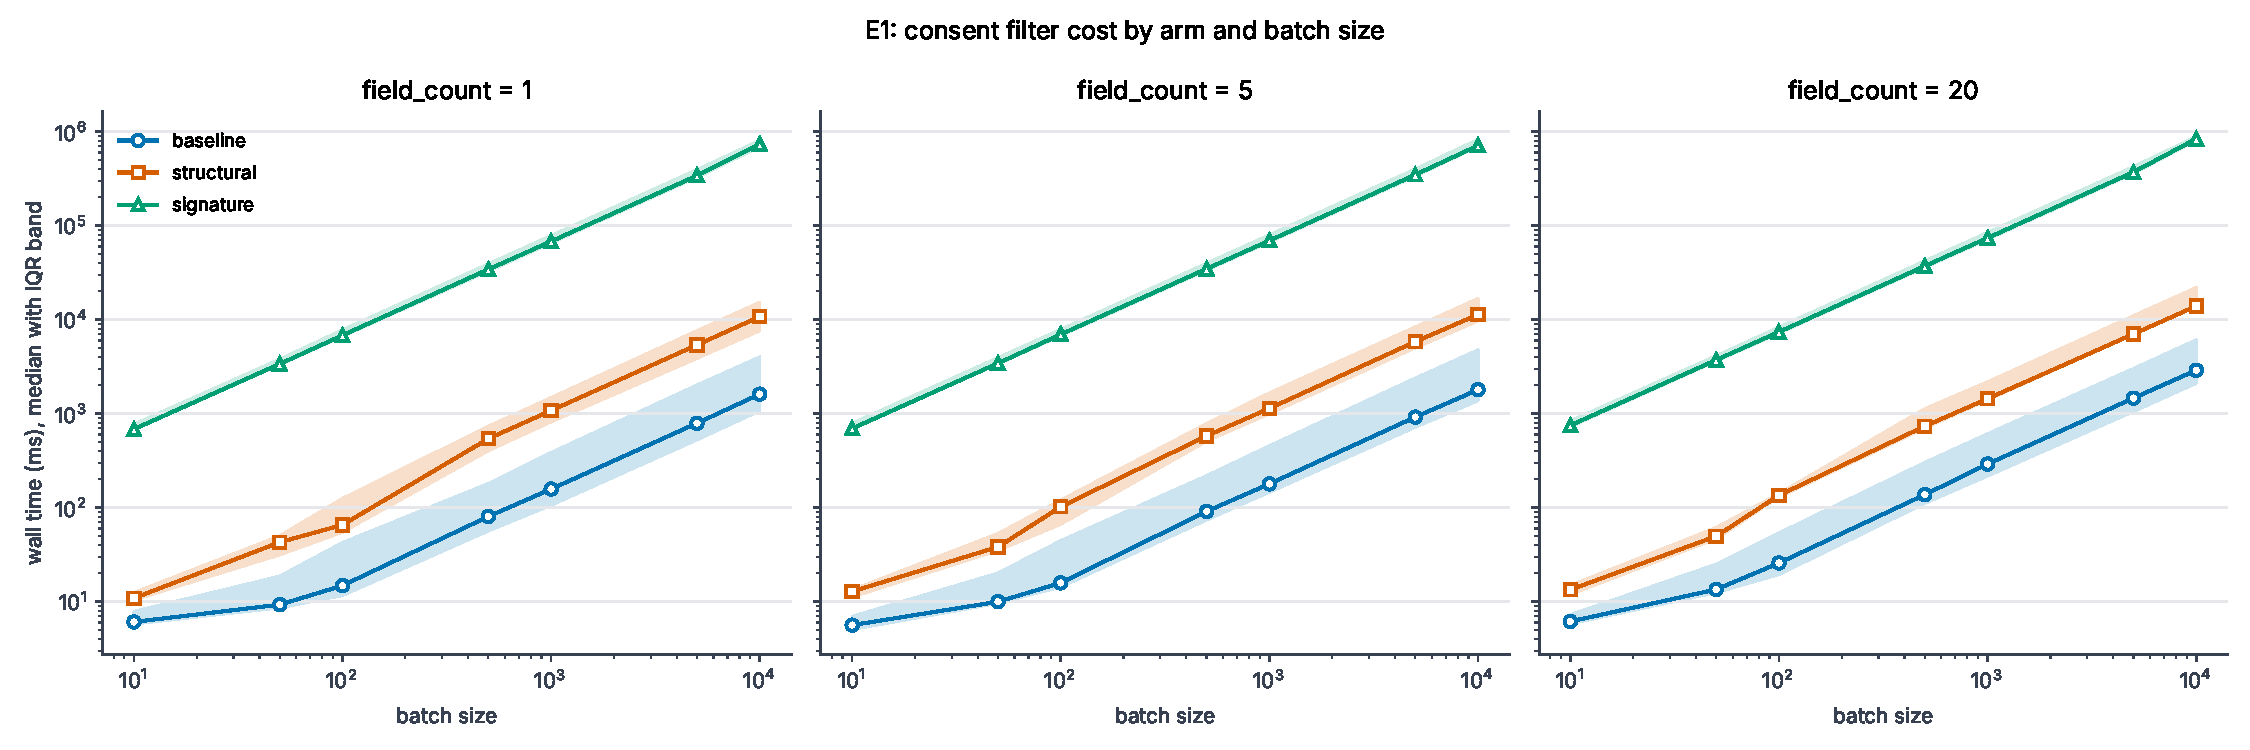
\includegraphics[width=0.9\linewidth]{../../experiments/analysis/figures/e1-crossover.pdf}
\caption{E1: signature-verification cost at the edge. Median wall time against batch size for the baseline, structural, and signature arms on log-log axes, one panel per field count (1, 5, 20). IQR bands shown for each arm.}
\end{figure}

Figure 1 (e1-crossover.pdf) plots median wall time against batch size for the three arms, baseline, structural, and signature, on log-log axes, one panel per field count. Across all three panels and the full swept batch-size range, from the smallest batch of 10 documents to the largest of 10,000, the three arms hold a fixed vertical ordering with no crossing: signature is costliest, structural is intermediate, and baseline is cheapest, at every plotted point.

At field\_count = 1 and the smallest swept batch (10 documents), median wall time is 6.07 ms (IQR 2.09 ms) for baseline, 10.85 ms (IQR 2.07 ms) for structural, and 682.41 ms (IQR 97.02 ms) for signature, a gap already present at the smallest batch the sweep tested: signature verification costs roughly 63 times the structural arm and 112 times the baseline arm at this point. The gap does not narrow as batch size grows. At the same field count and the largest swept batch (10,000 documents), median wall time is 1,607.78 ms (IQR 2,938.21 ms) for baseline, 10,735.27 ms (IQR 7,651.16 ms) for structural, and 731,749.77 ms (IQR 117,291.37 ms) for signature, a ratio of roughly 68 times structural and 455 times baseline. Across all three field counts and all seven batch sizes, the signature-to-structural ratio stays within a 50-to-104-fold band and the signature-to-baseline ratio within a 112-to-460-fold band. Neither ratio trends toward parity at any point in the swept range. At field\_count = 20, the largest field count tested, the pattern holds identically: signature median time runs from 748.32 ms at batch size 10 to 836,537.02 ms at batch size 10,000, remaining the costliest arm throughout. Table 3 gives the full field\_count = 1 sweep behind the two endpoints just quoted.

\begin{table}[H]
\caption{E1 wall time by batch size and arm, field\_count = 1, median (IQR) in milliseconds.\label{tab:t3}}
\small
\begin{tabular}{rrrr}
\toprule
Batch size & Baseline (ms) & Structural (ms) & Signature (ms) \\
\midrule
10 & 6.07 (IQR 2.09) & 10.85 (IQR 2.07) & 682.41 (IQR 97.02) \\
50 & 9.27 (IQR 10.05) & 42.75 (IQR 18.58) & 3,370.29 (IQR 478.45) \\
100 & 14.78 (IQR 30.81) & 65.38 (IQR 70.45) & 6,799.43 (IQR 1,147.54) \\
500 & 80.34 (IQR 123.86) & 540.02 (IQR 329.87) & 34,191.66 (IQR 6,511.47) \\
1,000 & 157.25 (IQR 278.55) & 1,076.41 (IQR 662.53) & 67,888.55 (IQR 13,159.07) \\
5,000 & 789.80 (IQR 1,487.63) & 5,372.79 (IQR 3,741.41) & 339,802.61 (IQR 66,529.45) \\
10,000 & 1,607.78 (IQR 2,938.21) & 10,735.27 (IQR 7,651.16) & 731,749.77 (IQR 117,291.37) \\
\bottomrule
\end{tabular}
\end{table}

There is no crossover point anywhere in the data. Signature verification is the dominant cost from the smallest batch onward, not a cost that overtakes the other arms past some threshold batch size. The three lines in Figure 1 run parallel on the log-log plot rather than intersecting.

The signature arm exists only inside E1's harness: it runs against a separate CouchDB design document (\texttt{build-signature-design-doc.ts}) that E1 builds and installs itself, never against the production \texttt{consent-couchdb} design document any real deployment's provisioning path installs. The production S1 filter performs no per-record signature verification of any kind. The three arms above measure what per-record signature verification would cost if it were added to the write path, not a cost the deployed system currently pays.

\subsection{E2: Revocation Propagation Under Network Partition}


\begin{figure}[H]
\centering
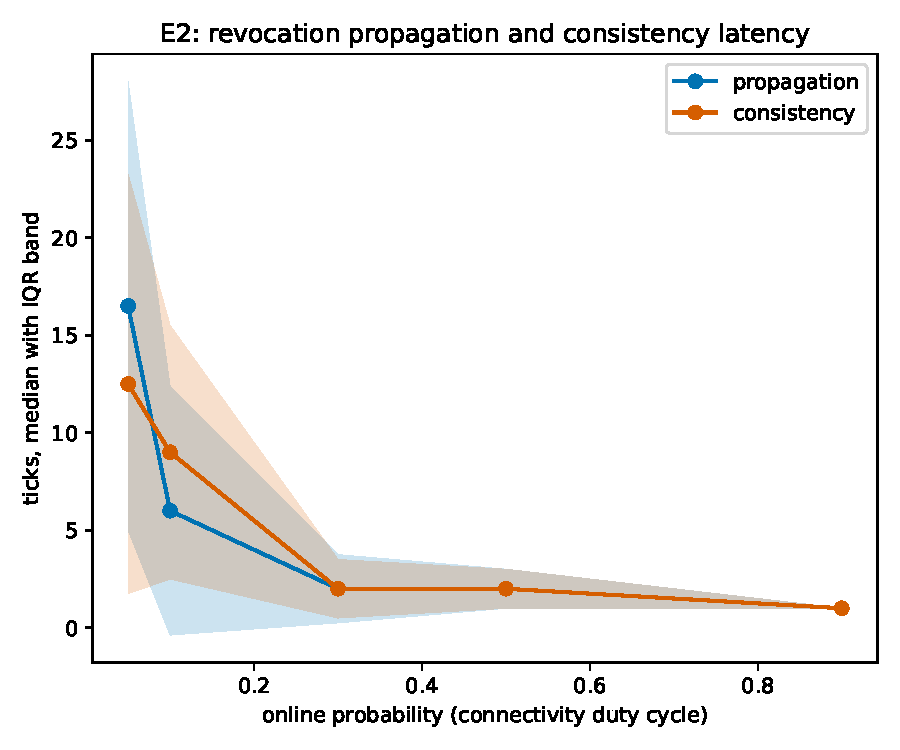
\includegraphics[width=0.9\linewidth]{../../experiments/analysis/figures/e2-propagation.pdf}
\caption{E2: revocation propagation and consistency latency against online probability, with IQR bands.}
\end{figure}

Figure 2 (e2-propagation.pdf) plots median propagation ticks and median consistency ticks against online probability, the duty-cycle parameter governing how often a simulated device comes online, swept across five values: 0.05, 0.1, 0.3, 0.5, and 0.9. Both curves fall sharply at low connectivity and flatten as connectivity increases. Median propagation ticks are 16.5 at online\_probability = 0.05, 6.0 at 0.1, 2.0 at 0.3, 2.0 at 0.5, and 1.0 at 0.9. Median consistency ticks follow a similar shape: 12.5 at 0.05, 9.0 at 0.1, 2.0 at 0.3, 2.0 at 0.5, and 1.0 at 0.9. Both series converge to the same value, 2.0 ticks, at online\_probability = 0.3 and 0.5, and both reach a floor of 1.0 tick at the highest tested connectivity, online\_probability = 0.9. The IQR bands are widest at the lowest connectivity value (propagation IQR of 23 ticks and consistency IQR of 21.5 ticks at online\_probability = 0.05) and narrow to zero by online\_probability = 0.9, reflecting the point at which nearly every device is online on nearly every tick. Table 4 gives the full sweep.

\begin{table}[H]
\caption{E2 propagation and consistency ticks by online probability, median (IQR).\label{tab:t4}}
\small
\begin{tabular}{rrrrr}
\toprule
Online probability & Prop. Median (ticks) & Prop. IQR & Cons. Median (ticks) & Cons. IQR \\
\midrule
0.05 & 16.5 & 23 & 12.5 & 21.5 \\
0.1 & 6 & 12.75 & 9 & 13 \\
0.3 & 2 & 3.5 & 2 & 3 \\
0.5 & 2 & 2 & 2 & 2 \\
0.9 & 1 & 0 & 1 & 0 \\
\bottomrule
\end{tabular}
\end{table}

Across all five sweep points, pooling 90 data points per point for both the revocation-device and conflict-device measurements (150 independent fleet trials in total, 30 per sweep point), the leaked-record count and the unresolved-conflict count are both 0. No trial, at any tested connectivity level including the most disconnected duty cycle tested (online\_probability = 0.05), produced a record visible in the shared CouchDB database for a purpose the owning participant had revoked, and no trial left an injected conflict unresolved by the end of its run.

\subsection{E3: Audit-Chain Verification Cost at Scale}


\begin{figure}[H]
\centering
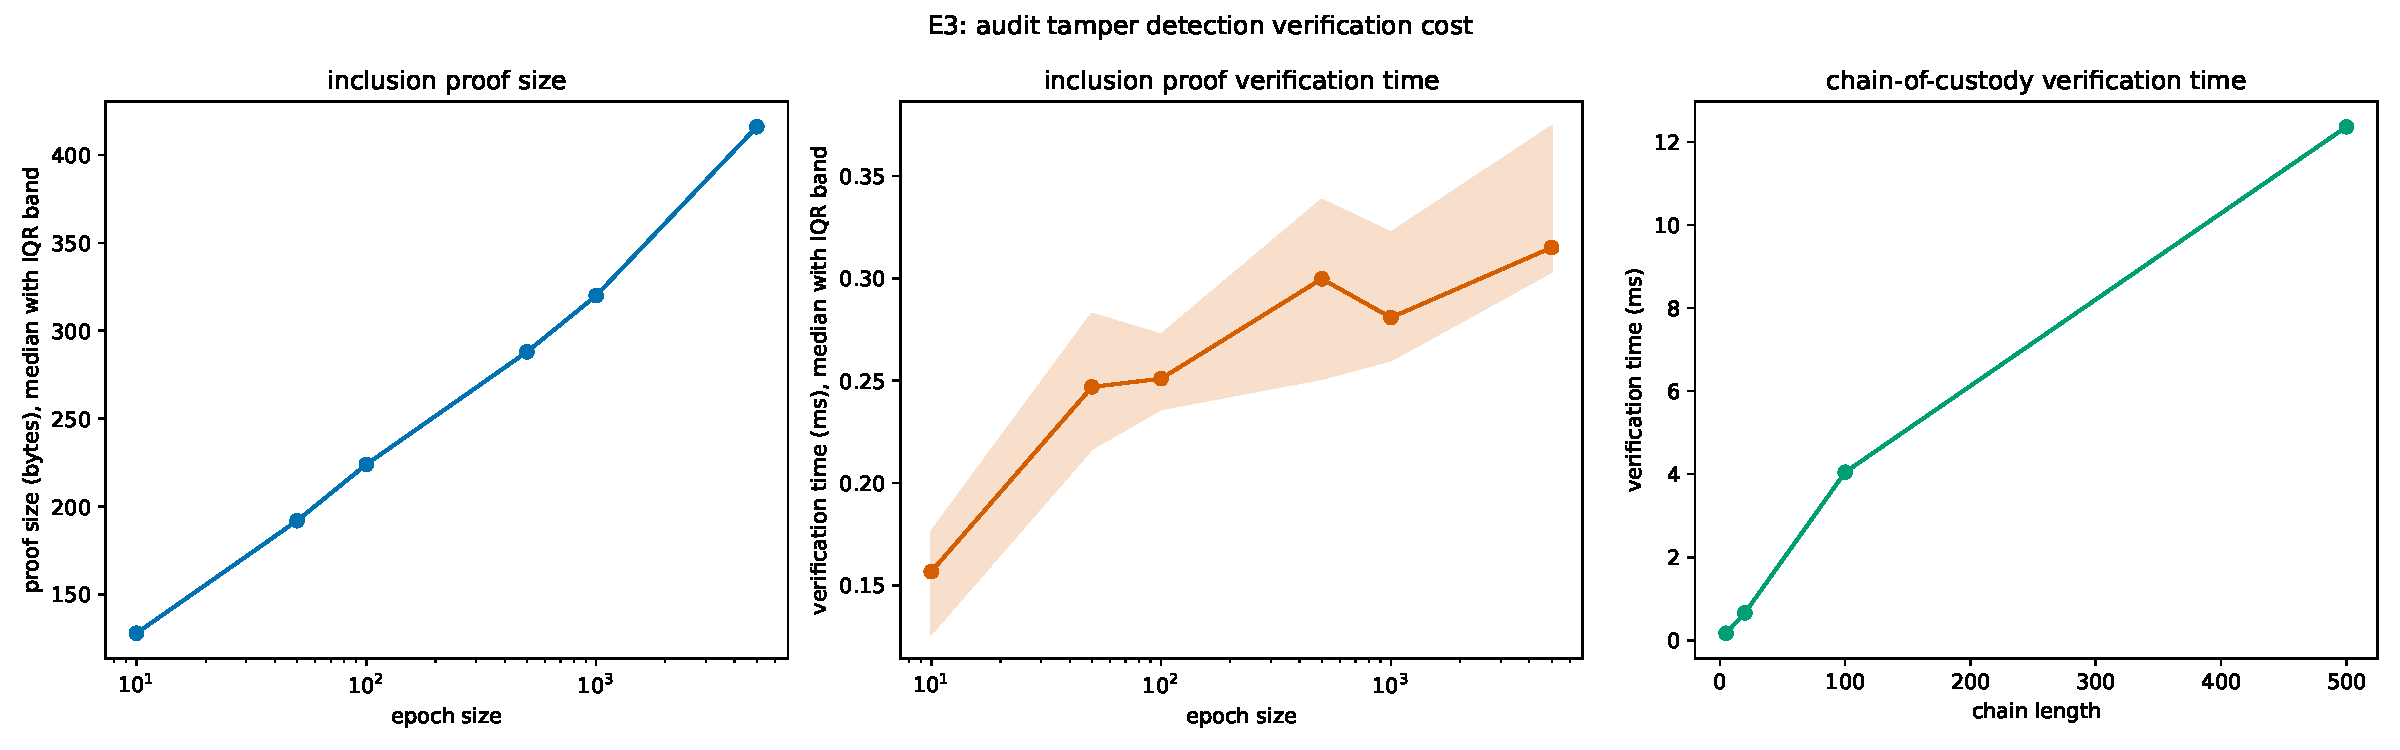
\includegraphics[width=0.9\linewidth]{../../experiments/analysis/figures/e3-verification-cost.pdf}
\caption{E3: audit-chain verification cost at scale. (\textbf{a}) Inclusion proof size against epoch size. (\textbf{b}) Inclusion-proof verification time against epoch size. (\textbf{c}) Chain-of-custody verification time against chain length.}
\end{figure}

Figure 3 (e3-verification-cost.pdf) presents three panels: inclusion proof size and inclusion-proof verification time, both swept against epoch size on a log x-axis, and chain-of-custody verification time swept against chain length.

Median proof size grows from 128 bytes at epoch\_size = 10 to 416 bytes at epoch\_size = 5000, passing through 192 bytes at epoch\_size = 50, 224 bytes at epoch\_size = 100, 288 bytes at epoch\_size = 500, and 320 bytes at epoch\_size = 1000. Median inclusion-proof verification time rises over the same sweep from 0.157 ms at epoch\_size = 10 to 0.315 ms at epoch\_size = 5000, with intermediate medians of 0.247 ms at epoch\_size = 50, 0.251 ms at epoch\_size = 100, 0.300 ms at epoch\_size = 500, and a slight dip to 0.281 ms at epoch\_size = 1000 before rising again at the largest epoch size. Every inclusion-proof verification measured across the full sweep stays under one millisecond. Chain-of-custody verification time, measured separately against chain length rather than epoch size since it depends only on the number of epochs to compare and not their internal size, rises from 0.169 ms at a chain length of 5 to 12.364 ms at a chain length of 500, passing through 0.660 ms at chain length 20 and 4.047 ms at chain length 100, each point the median of ten timed repetitions following an untimed warmup pass, the same protocol section 4.3 describes. Table 5 gives the epoch-size sweep and Table 6 the chain-length sweep behind these numbers.

\begin{table}[H]
\caption{E3 inclusion-proof size and verification time by epoch size, median (IQR).\label{tab:t5}}
\begin{tabularx}{\textwidth}{rrX}
\toprule
Epoch size & Proof size, median (bytes) & Inclusion verification, median ms (IQR) \\
\midrule
10 & 128 & 0.157 (IQR 0.049) \\
50 & 192 & 0.247 (IQR 0.065) \\
100 & 224 & 0.251 (IQR 0.036) \\
500 & 288 & 0.300 (IQR 0.087) \\
1,000 & 320 & 0.281 (IQR 0.062) \\
5,000 & 416 & 0.315 (IQR 0.071) \\
\bottomrule
\end{tabularx}
\end{table}

\begin{table}[H]
\caption{E3 chain-of-custody verification time by chain length, median of ten timed repetitions.\label{tab:t6}}
\small
\begin{tabular}{rr}
\toprule
Chain length & Verification time, median (ms) \\
\midrule
5 & 0.169 \\
20 & 0.660 \\
100 & 4.047 \\
500 & 12.364 \\
\bottomrule
\end{tabular}
\end{table}

Tamper detection itself is not a quantity this sweep measures. E3's harness times and sizes calls into audit-chain logic that an earlier implementation phase already tested at the boolean level, and it deliberately performs no tamper injection of its own. That earlier phase's own test suite (\texttt{MerkleTreeTest.java} and \texttt{packages/audit-verify}'s \texttt{chain.test.ts}) establishes 100\% tamper detection at the mechanism level: a wrong leaf, a mutated root, and a tampered proof step each fail inclusion verification, and a reordered or mutated-root epoch is caught by chain verification, in every case tested. E3's contribution is the cost curve layered on top of that already-established correctness result, not a re-measurement of detection accuracy itself.

\subsection{E4: Privacy-Budget-Versus-Utility Tradeoff}


\begin{figure}[H]
\centering
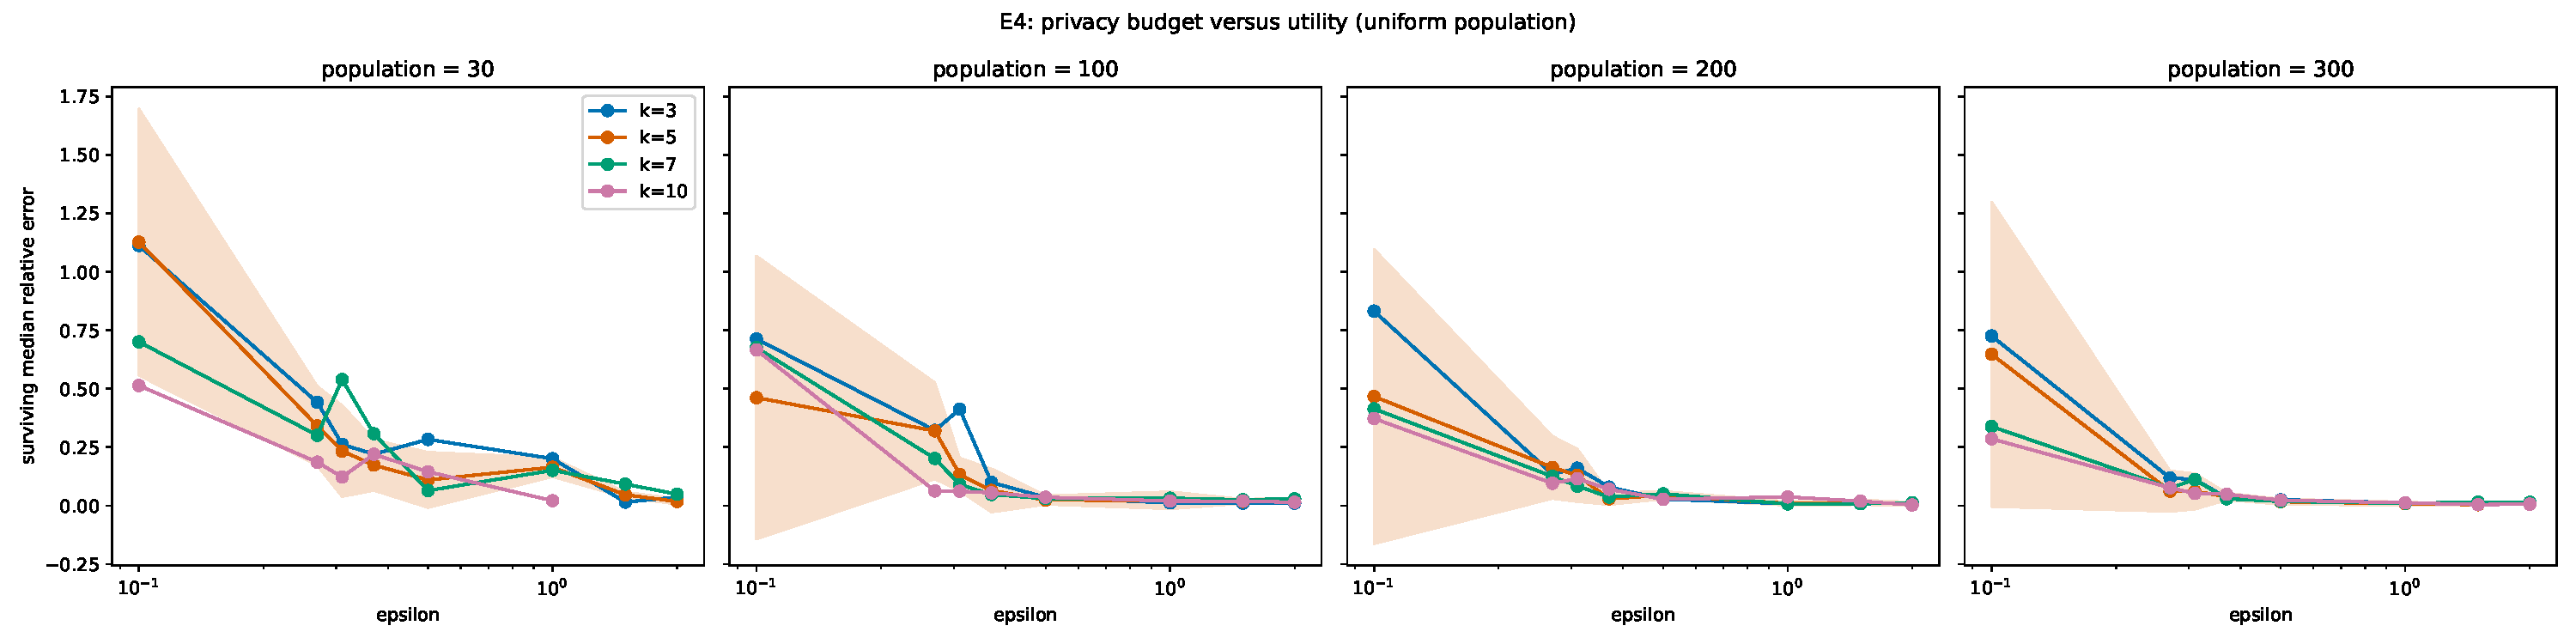
\includegraphics[width=0.9\linewidth]{../../experiments/analysis/figures/e4-utility.pdf}
\caption{E4: privacy-budget-versus-utility tradeoff. Surviving median relative error against epsilon, one panel per population size, one line per k threshold, uniform skew only.}
\end{figure}

Figure 4 (e4-utility.pdf) plots the surviving median relative error, computed only over query results that were neither k-anonymity suppressed nor budget refused, against epsilon on a log x-axis, one panel per population size (30, 100, 200, 300), one line per k threshold (3, 5, 7, 10), restricted to the uniform population-skew slice of the swept grid. The surviving-only statistic is used deliberately: the plain median-relative-error column is pinned at a sentinel value of 1.0 across nearly the entire swept grid, since it assigns that sentinel to every suppressed or refused group rather than reporting the accuracy of the answers that were actually returned, and would show a flat, uninformative line rather than the real accuracy-versus-epsilon relationship.

The dominant pattern across all four population panels is that surviving median relative error falls as epsilon rises, most steeply between epsilon = 0.1 and epsilon = 0.5, then flattening toward a low floor by epsilon = 1.0 and above. At population = 30, the smallest tested, surviving median relative error at epsilon = 0.1 ranges from 0.513 (k = 10, IQR 0.502) to 1.127 (k = 5, IQR 1.140) across the four k values, and falls to a range of 0.017 to 0.049 by epsilon = 2.0, though at that same population and epsilon the surviving-point counts are again thin, 5, 3, 3, and 0 of 68 across the four k values (k = 10 has no surviving points at all at this cell), so this epsilon = 2.0 accuracy floor carries the same thin-sample caveat as the epsilon = 0.1 figures below. At population = 300, the largest tested, the same statistic starts lower at epsilon = 0.1, ranging from 0.286 (k = 10, IQR 0.579) to 0.726 (k = 3, IQR 1.223), and falls to a range of 0.006 to 0.014 by epsilon = 2.0. Suppression is heaviest at the combination of small population and high k: at population = 30, k = 10, the suppression/refusal rate is 95.6\% at epsilon = 0.1 and reaches 100\% at epsilon = 1.5 and epsilon = 2.0, meaning zero surviving data points at those two grid cells and no surviving-error value to report there. At population = 300, suppression is markedly lighter at low epsilon: the suppression/refusal rate at epsilon = 0.1 ranges from 6.5\% (k = 3) to 56.1\% (k = 10), compared with 64.7\% to 95.6\% at population = 30 for the same k values. Table 7 gives these two population panels' endpoint epsilon values side by side, with the surviving-point count behind each figure.

\begin{table}[H]
\caption{E4 surviving median relative error at epsilon = 0.1 and epsilon = 2.0, uniform skew, median (IQR) [surviving points / total grid points].\label{tab:t7}}
\small
\begin{tabular}{rrrr}
\toprule
Population & k & epsilon = 0.1 & epsilon = 2.0 \\
\midrule
30 & 3 & 1.113 (IQR 1.798) [n=24/68] & 0.036 (IQR 0.087) [n=5/68] \\
30 & 5 & 1.127 (IQR 1.140) [n=13/68] & 0.017 (IQR 0.023) [n=3/68] \\
30 & 7 & 0.701 (IQR 0.383) [n=10/68] & 0.049 (IQR 0.070) [n=3/68] \\
30 & 10 & 0.514 (IQR 0.502) [n=3/68] & no surviving points [n=0/68] \\
300 & 3 & 0.726 (IQR 1.223) [n=100/107] & 0.008 (IQR 0.007) [n=5/107] \\
300 & 5 & 0.647 (IQR 1.304) [n=86/107] & 0.009 (IQR 0.009) [n=5/107] \\
300 & 7 & 0.338 (IQR 0.860) [n=62/107] & 0.014 (IQR 0.015) [n=5/107] \\
300 & 10 & 0.286 (IQR 0.579) [n=47/107] & 0.006 (IQR 0.004) [n=5/107] \\
\bottomrule
\end{tabular}
\end{table}

The population = 30, epsilon = 0.1 numbers just reported carry sharply unequal statistical weight across k, since the surviving-only statistic is computed only over the queries that were not suppressed or refused at that cell: the 0.513 figure for k = 10 is a median over 3 surviving data points out of 68, the k = 7 figure over 10, the k = 5 figure over 13, and the k = 3 figure over 24. A reader comparing 0.513 (k = 10) against 1.127 (k = 5) at this cell is comparing a statistic computed on 3 points against one computed on 13, not two equally-supported estimates, and the k = 10 figure in particular should be read as illustrative of the few queries that happened to clear suppression at that combination rather than as a stable estimate of typical accuracy there. The same caution applies wherever a low-epsilon, small-population, high-k cell is quoted elsewhere in this section or in Chapter 6.

\subsection{G1: Quorum Availability Under the Built Policy and the Veto Policy SIDS 2026 Specified}


\begin{figure}[H]
\centering
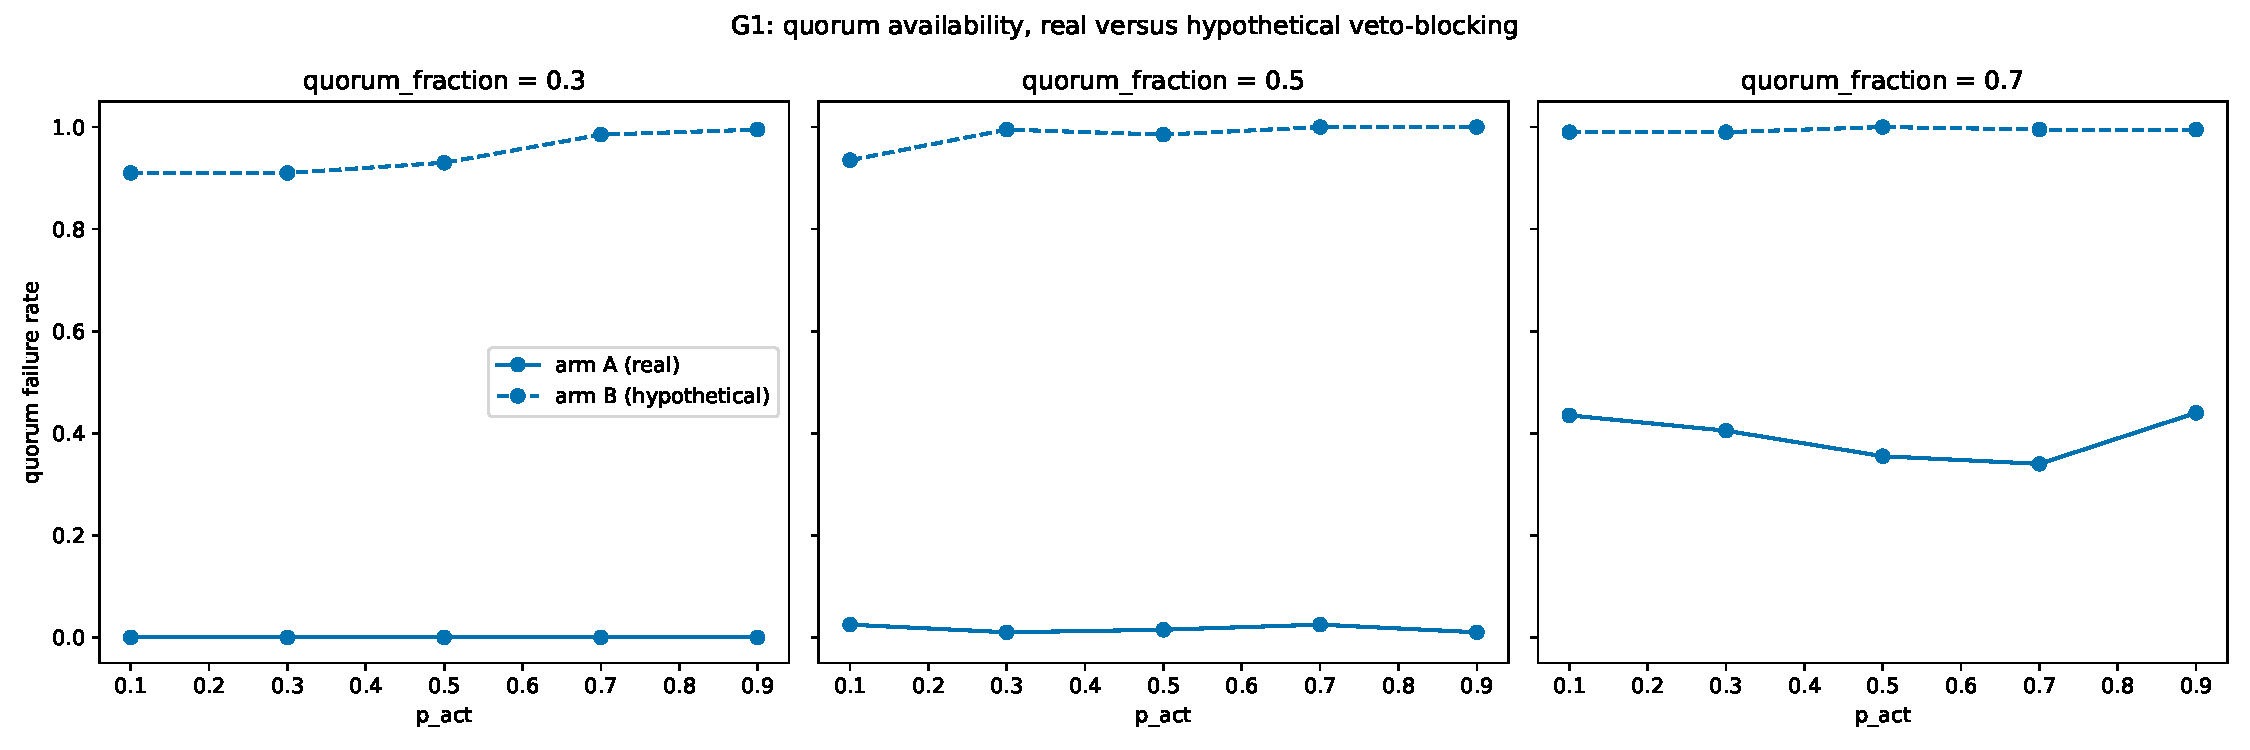
\includegraphics[width=0.9\linewidth]{../../experiments/analysis/figures/g1-availability.pdf}
\caption{G1: quorum failure rate against action probability for Arm A (the built, veto-blind policy) and Arm B (SIDS 2026's specified veto policy), one panel per quorum fraction.}
\end{figure}

Figure 5 (g1-availability.pdf) plots quorum failure rate against per-tick action probability (p\_act), one panel per quorum fraction (0.3, 0.5, 0.7), comparing two lines. Arm A drives the real, unmodified \texttt{StewardQuorumFunction}, the built system's policy: a release clears once the same swept quorum count Q has signed, and a recorded veto has no effect on that decision, matching section 3.4's disclosure. Arm B drives a second decision function that adds exactly the check SIDS 2026 specified and the built system omits: the identical swept quorum count Q as Arm A (SIDS 2026's own text names two-of-three co-signature as the specific case of this rule), plus a permanent block the moment any single steward vetoes, evaluated on the identical simulated timeline as Arm A so the only difference between the two lines is whether the veto SIDS 2026 promised is actually enforced. Arm A's failure rate is computed as 1 minus its reached rate. Arm B's is computed as its starved rate plus its vetoed rate, since Arm B's failures split across two mutually exclusive outcomes and its starved rate alone would omit its dominant failure mode. Both arms are shown at the filtered slice veto\_share = 0.3 and N = 20, the largest tested veto share and the largest tested steward pool, the combination that shows the clearest separation between the two policies. This slice yields 15 plotted points, five p\_act values across each of three quorum-fraction panels.

Framed this way, G1 does not compare the built system against an arbitrary stricter alternative. It measures the availability cost of enforcing the veto guarantee SIDS 2026 actually specified in its own text, a guarantee the implementation currently does not provide. Arm A fails far less often than Arm B at every one of the 15 plotted points, precisely because Arm A never lets a veto stop a release. At quorum\_fraction = 0.3, Arm A's failure rate is 0.0 across all five tested p\_act values (median ticks-to-quorum 1.0 to 6.0, IQR 0.0 to 3.0), while Arm B's failure rate ranges from 0.910 (p\_act = 0.1 and 0.3) to 0.995 (p\_act = 0.9). At quorum\_fraction = 0.5, Arm A's failure rate ranges from 0.010 to 0.025 (median ticks-to-quorum 1.0 to 12.0, IQR up to 7.0 at p\_act = 0.1), while Arm B's ranges from 0.935 to 1.0. At quorum\_fraction = 0.7, the panel with the narrowest gap, Arm A's failure rate ranges from 0.340 to 0.440 (median ticks-to-quorum 1.0 to 20.0, IQR up to 10.0 at p\_act = 0.1), while Arm B's ranges from 0.990 to 1.0. Table 8 gives all 15 plotted points, splitting each arm's failure rate into its component causes.

\begin{table}[H]
\caption{G1 quorum failure rate and its components, veto\_share = 0.3, N = 20.\label{tab:t8}}
\small
\begin{tabular}{rrrrrrr}
\toprule
Quorum frac. & p\_act & A fail rate & A starved rate & B fail rate & B vetoed rate & B starved rate \\
\midrule
0.3 & 0.1 & 0.000 & 0.000 & 0.910 & 0.910 & 0.000 \\
0.3 & 0.3 & 0.000 & 0.000 & 0.910 & 0.910 & 0.000 \\
0.3 & 0.5 & 0.000 & 0.000 & 0.930 & 0.930 & 0.000 \\
0.3 & 0.7 & 0.000 & 0.000 & 0.985 & 0.985 & 0.000 \\
0.3 & 0.9 & 0.000 & 0.000 & 0.995 & 0.995 & 0.000 \\
0.5 & 0.1 & 0.025 & 0.025 & 0.935 & 0.935 & 0.000 \\
0.5 & 0.3 & 0.010 & 0.010 & 0.995 & 0.995 & 0.000 \\
0.5 & 0.5 & 0.015 & 0.015 & 0.985 & 0.985 & 0.000 \\
0.5 & 0.7 & 0.025 & 0.025 & 1.000 & 1.000 & 0.000 \\
0.5 & 0.9 & 0.010 & 0.010 & 1.000 & 1.000 & 0.000 \\
0.7 & 0.1 & 0.435 & 0.435 & 0.990 & 0.990 & 0.000 \\
0.7 & 0.3 & 0.405 & 0.405 & 0.990 & 0.990 & 0.000 \\
0.7 & 0.5 & 0.355 & 0.355 & 1.000 & 1.000 & 0.000 \\
0.7 & 0.7 & 0.340 & 0.340 & 0.995 & 0.995 & 0.000 \\
0.7 & 0.9 & 0.440 & 0.440 & 0.995 & 0.995 & 0.000 \\
\bottomrule
\end{tabular}
\end{table}

Computed pointwise across all 15 plotted points, the divergence between Arm B's failure rate and Arm A's failure rate has a minimum of 0.555, occurring at quorum\_fraction = 0.7, and a maximum of 0.995, occurring at quorum\_fraction = 0.3, p\_act = 0.9. At no plotted point does the gap between the two arms fall below 0.555: enforcing the veto SIDS 2026 specified would raise the quorum failure rate far above what the built, veto-blind policy currently exhibits at every combination of quorum fraction and action probability tested.

Splitting Arm B's failure rate into its two mutually exclusive components at this same slice shows that the gap is driven almost entirely by vetoes rather than by genuine starvation. At all 15 plotted points, \texttt{arm\_b\_starved\_rate} is 0.0: no run in this slice reaches \texttt{maxTicks} without either quorum or a veto. \texttt{arm\_b\_vetoed\_rate} alone accounts for the entire failure rate reported above, from 0.910 at quorum\_fraction = 0.3, p\_act = 0.1, to 1.0 at several points in the quorum\_fraction = 0.5 and 0.7 panels (for example quorum\_fraction = 0.5, p\_act = 0.7 and 0.9, and quorum\_fraction = 0.7, p\_act = 0.5). This means Arm B's high failure rate is not evidence that the veto-enforcing policy is prone to stalling independently of stewards' objections. It is a direct, mechanical consequence of a 0.3 veto share applied across a pool of 20 stewards, where enough stewards act that at least one veto lands before quorum is reached almost every time. The veto mechanism, when actually enforced, works as specified: it blocks release whenever a steward objects. What the data show is the availability price of that guarantee at this veto share, not a separate defect in the quorum-reaching logic itself. Arm A, by contrast, does exhibit genuine starvation at the higher quorum fractions independent of any veto, since it ignores vetoes entirely: \texttt{arm\_a\_starved\_rate} reaches 0.435 at quorum\_fraction = 0.7, p\_act = 0.1, reflecting only that not enough stewards signed within the 200-tick horizon, the one failure mode Arm A can have.

\subsection{G2: Consent Heterogeneity Versus Aggregate Utility}


\begin{figure}[H]
\centering
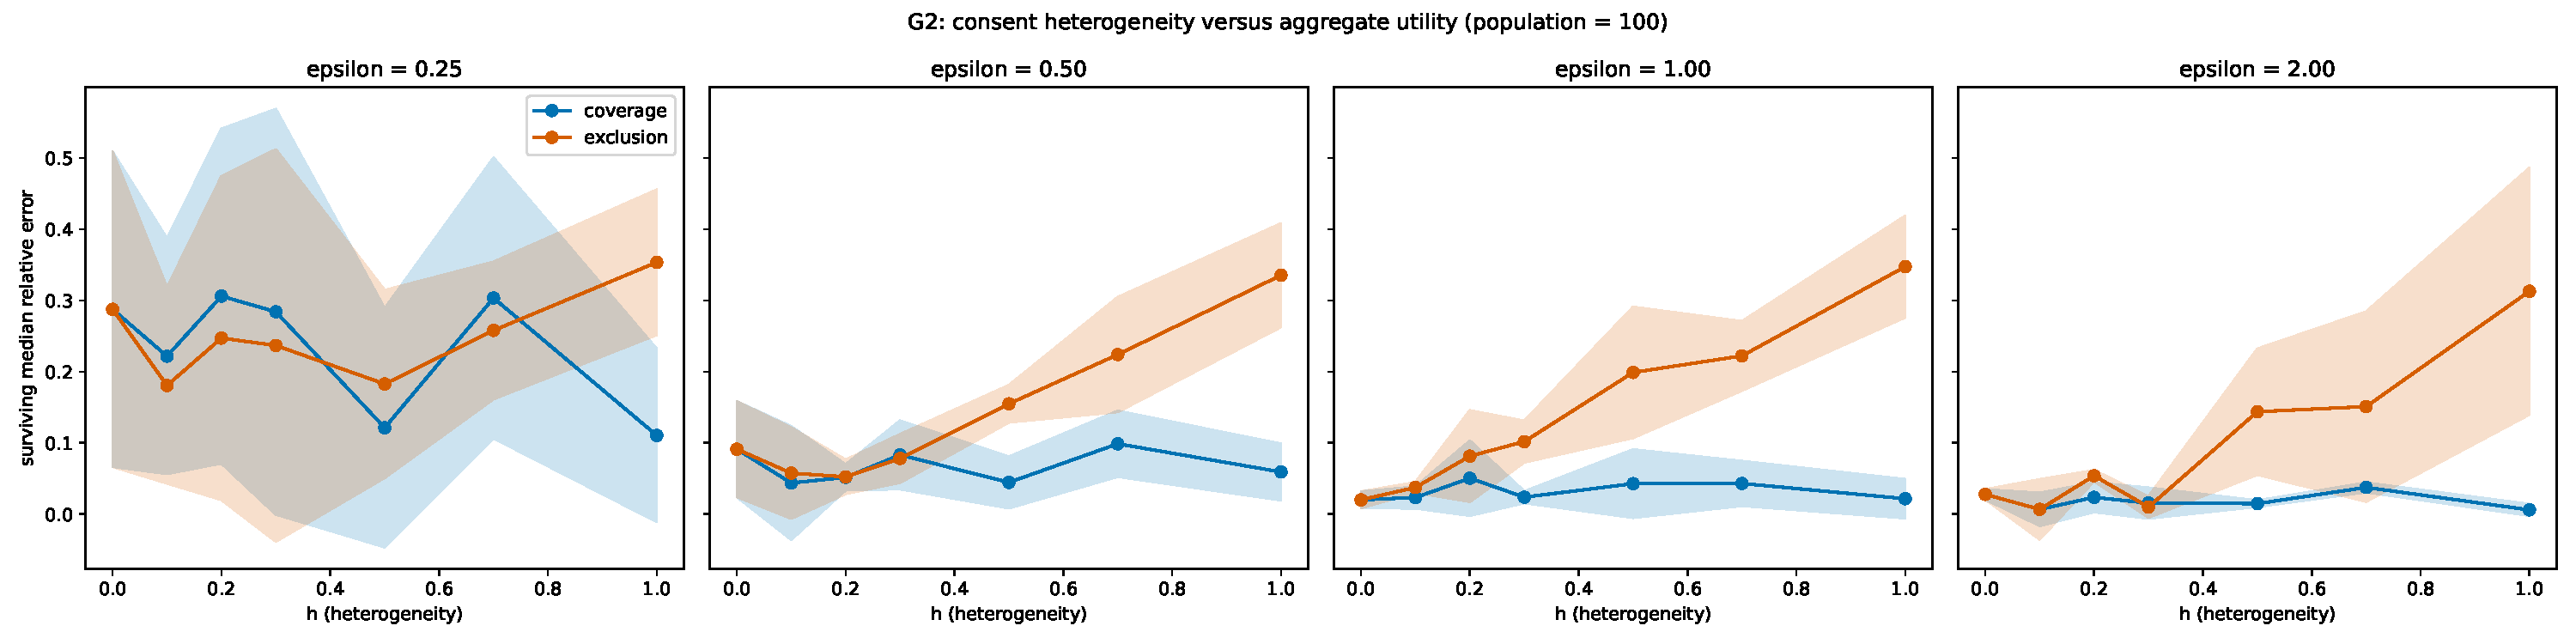
\includegraphics[width=0.9\linewidth]{../../experiments/analysis/figures/g2-heterogeneity.pdf}
\caption{G2: surviving coverage error and surviving exclusion error against consent heterogeneity h, one panel per epsilon, with IQR bands.}
\end{figure}

Figure 6 (g2-heterogeneity.pdf) plots two surviving-only relative-error statistics against heterogeneity h, one panel per epsilon (0.25, 0.5, 1.0, 2.0), restricted to population = 100. Both statistics are computed from the same noised \texttt{PrivacyPipeline.compute()} output. They differ only in which ground truth that noised output is compared against. Surviving coverage error compares the observed, noised result against the consenting population's own true count, so the consenting population is already the reference: this statistic isolates the DP mechanism's own noise, since the population it is measured against has already had heterogeneous consent's exclusions applied to it before the comparison is made. Surviving exclusion error compares the same observed, noised result against the full generated population's true count, unfiltered by consent: this statistic captures total distortion against the true community value, noise and exclusion bias together, not exclusion bias in isolation and not a quantity computed before noise is applied. It is the gap between exclusion error and coverage error, not exclusion error alone, that isolates the effect of heterogeneous consent specifically, since that gap is exactly the part of the total distortion coverage error's noise-only comparison does not already account for. As with E4, the surviving-only columns are used because the plain coverage- and exclusion-error columns are pinned at a sentinel value across most of the swept grid.

At epsilon = 1.0, surviving exclusion error rises from 0.020 (IQR 0.023) at h = 0.0 to 0.348 (IQR 0.142) at h = 1.0, passing through 0.037 at h = 0.1, 0.081 at h = 0.2, 0.102 at h = 0.3, 0.199 at h = 0.5, and 0.222 at h = 0.7, a roughly seventeen-fold increase across the heterogeneity sweep. At epsilon = 2.0, exclusion error also ends far above where it starts, rising from 0.028 at h = 0.0 to 0.313 at h = 1.0, though the path between those endpoints is not strictly monotonic: it dips to 0.007 at h = 0.1 and to 0.010 at h = 0.3 before climbing through 0.144 at h = 0.5 and 0.151 at h = 0.7 on the way to the h = 1.0 maximum. Surviving coverage error over the same two epsilon values shows no comparable overall trend: at epsilon = 1.0 it ranges narrowly from 0.020 (IQR 0.023) to 0.050 (IQR 0.105 at h = 0.2) across the full h sweep with no monotonic direction, and at epsilon = 2.0 it ranges from 0.006 to 0.037, again without trending upward as h increases. At the lowest tested epsilon (0.25), where Laplace noise is largest, both statistics are noisier and the separation is less clean, coverage error ranges from 0.111 to 0.306 (IQR from 0.243 to 0.569 across the sweep) and exclusion error from 0.181 to 0.354 (IQR from 0.193 to 0.550), but exclusion error still reaches its sweep maximum at h = 1.0 (0.354) while coverage error does not show the same endpoint behavior (0.111 at h = 1.0, within the range seen at smaller h values). Because coverage error stays flat while exclusion error climbs, the gap between them, not exclusion error by itself, is the cleanest read of heterogeneity's own effect: at epsilon = 1.0 that gap widens from effectively 0.0 at h = 0.0 (where the two statistics are identical by construction) to roughly 0.326 at h = 1.0 (0.348 exclusion against 0.022 coverage), tracking the growth in excluded\_fraction reported below rather than any change in the noise mechanism itself. Read this way, G2's finding is more precise than "exclusion error grows with heterogeneity" alone: it is that heterogeneous consent introduces a distortion on top of DP noise, one that grows with h, while the DP mechanism's own noise contribution, measured by coverage error, does not. Table 9 gives the full h sweep at epsilon = 1.0 and epsilon = 2.0, alongside the excluded fraction reported below.

\begin{table}[H]
\caption{G2 surviving coverage and exclusion error by heterogeneity h, population = 100, median (IQR).\label{tab:t9}}
\small
\begin{tabular}{rrrrrr}
\toprule
h & Excl. Frac. & eps=1.0 cov. & eps=1.0 excl. & eps=2.0 cov. & eps=2.0 excl. \\
\midrule
0.0 & 0.00 & 0.020 (IQR 0.023) & 0.020 (IQR 0.023) & 0.028 (IQR 0.014) & 0.028 (IQR 0.014) \\
0.1 & 0.08 & 0.023 (IQR 0.030) & 0.037 (IQR 0.015) & 0.007 (IQR 0.046) & 0.007 (IQR 0.084) \\
0.2 & 0.16 & 0.050 (IQR 0.105) & 0.081 (IQR 0.128) & 0.024 (IQR 0.041) & 0.054 (IQR 0.015) \\
0.3 & 0.27 & 0.024 (IQR 0.016) & 0.102 (IQR 0.058) & 0.015 (IQR 0.043) & 0.010 (IQR 0.030) \\
0.5 & 0.49 & 0.043 (IQR 0.096) & 0.199 (IQR 0.184) & 0.015 (IQR 0.009) & 0.144 (IQR 0.177) \\
0.7 & 0.73 & 0.043 (IQR 0.063) & 0.222 (IQR 0.097) & 0.037 (IQR 0.013) & 0.151 (IQR 0.267) \\
1.0 & 1.00 & 0.022 (IQR 0.055) & 0.348 (IQR 0.142) & 0.006 (IQR 0.016) & 0.313 (IQR 0.346) \\
\bottomrule
\end{tabular}
\end{table}

The excluded fraction, the direct measurement of how much of the population lacked a valid grant for at least one query attribute, rises monotonically with h independent of epsilon: 0.0 at h = 0.0, 0.08 at h = 0.1, 0.16 at h = 0.2, 0.27 at h = 0.3, 0.49 at h = 0.5, 0.73 at h = 0.7, and 1.0 at h = 1.0.

\section{Discussion}

\subsection{Two Lines of Evidence, Not One}

SIDS 2026 \cite{katrakazas2026} reported that participants who used a co-designed prototype trusted the idea of observable sovereignty controls: a self-report finding, drawn from a sample of 23 participants, that people responded positively to being shown what a system claimed it would do. That finding says something real about uptake and legitimacy, and nothing directly about whether the mechanisms those participants were shown actually behave the way the design says they do under load, under partition, or under an adversarial steward. The six experiments reported in Chapter 5 answer a different question: not whether people trust the architecture, but what the architecture, as built, actually guarantees, and at what cost.

It would overstate this paper's contribution to claim these two facts converge into a single, stronger proof of sovereignty. They do not measure the same thing, and a reviewer would be right to notice if the paper tried to make them look like they did. SIDS 2026's n=23 trust score is evidence that the promise of sovereignty controls is legible and credible to the people it is meant to serve. This paper's mechanism-level results are evidence that, independent of anyone's belief about them, the promised controls do what they claim under the conditions tested, sometimes at a cost participants were never shown a number for. The correct framing is complementary, not corroborating: two separate legs of one larger sovereignty argument, one subjective and participant-facing, one objective and mechanism-facing, neither one substituting for the other. A system could pass every experiment in Chapter 5 and still fail to earn trust in the field, for reasons the trust study is better positioned to capture than a wall-clock benchmark ever could. Equally, a system could earn high trust scores from participants shown a prototype and still leak revoked records under partition, refuse too many statistics to be useful, or grant a steward veto that nobody can actually exercise when it matters, none of which self-report can catch. Holding the two lines of evidence apart, rather than blending them, is itself the honest position this paper takes, and it is the same posture the project adopted when it corrected the steward-quorum claim discussed below rather than letting the original design description stand uncontested.

\subsection{Returning to the Open Governance Challenges}

SIDS 2026 closed with four open governance challenges that its own qualitative evaluation and design specification could name but not settle empirically, because the mechanisms behind them were not yet built. Chapter 5's experiments give three of those four challenges a real measurement to stand on. The fourth remains, honestly, outside what this paper measured.

\textbf{Privacy budget and community data utility.} SIDS 2026 stated a concern in general terms: differential privacy at $\varepsilon = 0.5$ per query and $\varepsilon_{\text{total}} = 2.0$ per site "can render aggregate statistics analytically meaningless at the low population volumes of individual service sites," and proposed exploring adaptive budgets and scenario-based community deliberation as a response, without a measurement to anchor the discussion. E4 supplies that measurement, at least for the epsilon and population ranges tested, and SIDS 2026's own operating point, $\varepsilon = 0.5$ per query, falls squarely inside the range E4 shows to be the steepest part of the accuracy curve: surviving median relative error falls most sharply between epsilon 0.1 and 0.5, before flattening toward a low floor from epsilon 1.0 upward, which means the exact budget SIDS 2026 proposed sits on the part of the curve where a small change in epsilon buys the largest change in usable accuracy. At the smallest population tested (30) and the tightest epsilon tested (0.1), surviving median relative error ranges from 0.513 to 1.127 across the four k thresholds, an error band that would make most service-level aggregates unusable for advocacy, exactly the failure mode SIDS 2026 worried about in the abstract. E4 also shows the concern is not uniform across the design space: at population 300, the same epsilon and k range starts substantially lower, 0.286 to 0.726, and both population sizes fall to a low floor, under 0.05 relative error at population 30 and under 0.015 at population 300, once epsilon rises to 2.0, though the population-30 floor rests on as few as 3 surviving data points out of 68 at some k values and none at all for k = 10, so it should be read as illustrative rather than a stable estimate (section 5.4 gives the exact counts). Suppression tells the same story from the other side: at population 30, k = 10, the suppression/refusal rate is 95.6\% at epsilon = 0.1, rising to 100\% by epsilon = 1.5, meaning most or all query attempts return nothing at all at exactly the small-site, tight-budget combination SIDS 2026 flagged.

G2 adds a second utility threat SIDS 2026's own framing did not anticipate, because it concerns consent heterogeneity rather than the epsilon budget itself. Holding epsilon fixed at 1.0, surviving exclusion error, which captures noise and exclusion bias together against the full-population ground truth, rises roughly seventeen-fold across the heterogeneity sweep, from 0.020 at h = 0.0 to 0.348 at h = 1.0, while surviving coverage error, which isolates the privacy mechanism's own noise and suppression behavior against the consenting population alone, stays flat over the same range, 0.020 to 0.050, with no comparable trend. Since exclusion error nests coverage error's noise component, it is the widening gap between the two, not exclusion error alone, that is attributable specifically to heterogeneous consent. The excluded fraction itself, the direct share of the population lacking a valid grant for at least one query attribute, rises monotonically with heterogeneity independent of epsilon, reaching 1.0 at h = 1.0. Read together with E4, this means the "aggregate too thin to be useful" worry SIDS 2026 raised has two distinct causes in the built system: privacy noise and suppression at low epsilon and small population (E4), and exclusion bias from heterogeneous consent grants that grows independently of epsilon (G2). A community deliberation process built only around explaining epsilon, as SIDS 2026's adaptive-budget proposal frames it, would not surface the second mechanism at all. Consent heterogeneity, not the privacy budget, is what drives it.

Rogers et al.'s (2021) LinkedIn budget accountant and Abowd et al.'s (2022) Census TopDown system are both real, deployed formal-privacy budgets with documented accuracy costs, but at population scales far above anything E4 tests: LinkedIn's audience-engagement queries and the U.S. Census both operate over populations many orders of magnitude larger than the 30-to-300 range that spans an individual service site. E4 sits in the gap between those two deployment reports and the small-population, single-site regime SIDS 2026's own governance challenge is actually about, and its numbers speak to a scale neither of those two systems' published results directly cover.

\textbf{Sustainable steward governance and sovereignty vs. institutional accountability.} SIDS 2026 named this tension directly: "A steward veto on outcomes data deprives institutions of needed monitoring information. Conversely, embedding stewards in institutional structures compromises their independence." G1 gives the first half of that sentence a number. Arm B in G1 is not a hypothetical stricter policy invented for comparison. It is SIDS 2026's own specified steward gate, "any single steward may veto, in which case the release request is returned to the requester with a written justification" \cite{katrakazas2026}, the same guarantee section 3.4 shows the built system's Arm A never checks. G1 therefore measures the availability cost of actually enforcing the veto SIDS 2026 already promised, not the cost of a stricter alternative the design considered and rejected. At the filtered slice that shows the clearest separation between the two, veto\_share = 0.3, N = 20, enforcing the veto (Arm B) raises the quorum failure rate far above the built system's current, veto-blind rate (Arm A) at every one of the 15 plotted combinations of quorum fraction and action probability, with the gap never smaller than 0.555 and reaching as high as 0.995. At quorum\_fraction = 0.3, Arm A never fails across the tested range, while Arm B fails 91.0 to 99.5\% of the time. Decomposing Arm B's failures shows this cost is not genuine quorum starvation: at every one of the 15 plotted points its starved rate is 0.0, and its entire failure rate is vetoed rate, a direct, mechanical consequence of a 0.3 veto share across a pool of 20 stewards, not evidence that a veto-enforcing policy stalls independently of stewards' actual objections. This does not settle the normative question SIDS 2026 raised, how much institutional monitoring access is worth how much steward leverage, which remains a governance choice rather than a technical one, but it gives the people who have to make that choice, including the three-country pilot's own comparison of stipend, in-kind, and institutional-embedding sustainability models, a real number for what enforcing the already-published veto guarantee would cost, rather than the false reassurance that the currently unenforced policy already represents a validated design choice. It also bears on sustainable governance in a narrower sense: a fully enforced veto policy gives stewards, particularly stipend-supported or part-time ones, a real blocked-release backlog to manage once vetoes actually stop a release, a workload cost the pilot's stipend-model comparison did not previously have a mechanism-level number to weigh against.

\textbf{Multi-channel sovereignty equivalence.} SIDS 2026's liaison-accountability protocol for paper-form submissions, SMS-confirmed digitization acknowledgment, liaison-level audit logging, and participant-accessible retention of paper originals, has no corresponding experiment in this paper. None of the six experiments touch the liaison-digitization path, and no component of the built system described in Chapter 3 implements or simulates it. The audit-chain experiments (E3) measure proof size and verification time for entries already in the system, which says nothing about whether a liaison's transcription of a paper form into that system preserved the participant's actual intent at the point of digitization. Closing this gap would require a different kind of study, one centered on the liaison interaction itself, not a mechanism-level benchmark of the kind this paper runs. It remains open, and this chapter does not force a connection where none exists.

\subsection{The Steward-Quorum Gaps and What "Verified, Not Architected" Requires}

Section 3.4 already states the central correction this paper has to make about its own system: SIDS 2026 described the steward-release gate as a cryptographic envelope, aggregated outputs encrypted under a key reconstructable only from a quorum of steward signatures, and the design specification that followed initially retained Shamir secret sharing as a second lock on release precisely because a policy check the connector operator runs is a weaker guarantee than a cryptographic impossibility. What was actually built and verified against a running connector is \texttt{StewardQuorumFunction}, an ODRL constraint function that counts distinct steward signatures on a \texttt{StewardAuthorization} record and refuses contract negotiation unless that count meets a threshold. It is a real, negotiation-blocking gate, not a decorative one, but it is enforced by the software the connector operator runs, not by mathematics that holds regardless of who operates that software.

A second gap sits alongside the cryptographic one, and it is the more serious of the two. Section 3.4 discloses it directly: SIDS 2026's own text specifies not just a quorum but a veto, "any single steward may veto, in which case the release request is returned to the requester with a written justification" \cite{katrakazas2026}, and \texttt{StewardQuorumFunction.evaluate} never reads \texttt{authorization.vetoes()}. A recorded veto has no effect on whether a release clears contract negotiation. This gap is more serious than the cryptographic one not because it costs more in absolute terms, but because it diverges from a guarantee SIDS 2026 already published to its readers, rather than from an internal design intent that a reference implementation stopped short of realizing. G1 (section 5.5) gives this gap a measured cost rather than leaving it a qualitative disclosure: at the slice with the clearest separation, enforcing the veto SIDS 2026 specified would raise the quorum failure rate by at least 0.555 and as much as 0.995 above what the built system's veto-blind policy currently exhibits, and that cost is driven almost entirely by vetoes firing as designed rather than by genuine quorum starvation, since Arm B's starved rate is 0.0 at every plotted point in that slice. The steward-quorum limitation this paper discloses is therefore two gaps, not one: a cryptographic-envelope gap between the policy-engine check that was built and the threshold-decryption envelope SIDS 2026 described, and a veto-checking gap between the guarantee SIDS 2026 published and what the release decision actually consults.

This chapter's job is to say what these gaps mean, beyond restating that they exist. A paper whose thesis is that mechanism-level measurement should replace unverified architectural claims cannot itself carry an unverified architectural claim about one of its own central mechanisms. If this paper described the steward gate as cryptographic threshold decryption while the code implements a signature-count check, it would be doing exactly what SIDS 2026's own "Technical Implementation Status" section was careful not to do: describing a design as though it were the built system, rather than naming the gap between the two. The honest path, taken here and in Section 3.4, is to report the mechanism for what it is: real, load-bearing, and weaker than originally specified, rather than smoothing the distance between the two into a shared vocabulary that makes them sound equivalent. \cite{albalwy2026} offers a useful contrast from a comparable domain: ZK-EHR replaces an asserted governance property (a requester's policy compliance) with one verified through zero-knowledge proofs, checkable by any party without trusting the operator who runs the check. That is the general move this paper's own thesis argues for, measuring what a system actually guarantees rather than what it claims to. The cryptographic-envelope gap is the place in this reference implementation where that move has not yet been completed: the quorum guarantee is checked, but only by the party operating the check, not proven to an independent verifier the way Albalwy's zero-knowledge approach or Kokoris-Kogias et al.'s (2020) CALYPSO threshold decryption would allow. The veto-checking gap is a different kind of incompleteness, not a missing independence property but a missing check: the mechanism to honor SIDS 2026's promised veto already exists in \texttt{StewardAuthorization}'s \texttt{vetoes} list, and simply is not consulted.

Closing the cryptographic gap is a concrete, scoped engineering task, not a redesign. Section 3.4 already sets out the two closest comparators, CALYPSO's genuine threshold decryption benchmarked against committee size and Raisaro et al.'s (2019) MedCo, where decryption requires collective participation from every federated site holding a key share. Either pattern, applied here, would replace the current signature-count check with a real threshold-decryption step, \texttt{ReleaseArtifact} bytes encrypted under a key that only a quorum of stewards can jointly reconstruct, so that no connector operator, however configured, can produce plaintext without that quorum's actual cryptographic participation. The auditable structure this implementation already has, signed authorizations bound to a specific dataset hash, with separate review, veto, and appeal records, is compatible with that upgrade. It would sit alongside the cryptographic gate rather than being replaced by it. What is missing is the independence of the guarantee from the software making the check, which is precisely the property CALYPSO and MedCo hold and this implementation does not yet.

\subsection{E1 and the Absence of a Crossover}

Chapter 5 reported E1's result carefully: across every field count and every batch size swept, from 10 documents to 10,000, signature verification is the costliest of the three arms and structural checking the second costliest, with no crossover anywhere in the data. E1's signature arm runs only inside its own harness, against a separate CouchDB design document E1 builds and installs itself, not against the production \texttt{consent-couchdb} design document any real deployment provisions. The production S1 filter performs no per-record signature verification at all, so E1 measures what per-record signature verification would cost if it were added to the write path, not a cost the deployed system currently pays. That measured cost is worth stating plainly on its own terms: a fixed per-signature cost might, in principle, eventually be outrun by a cost that scales worse with batch size, producing a crossover point past which structural or baseline validation becomes the bottleneck instead. The measured data show no such crossover anywhere in the swept range. The signature-to-structural ratio stays within a 50-to-104-fold band across the entire swept range, and the signature-to-baseline ratio within a 112-to-460-fold band. Neither ratio drifts toward parity as batch size grows, because the pure-JavaScript Ed25519 implementation E1's harness measures scales with the number of documents at roughly the same rate the other arms do, just with a much larger constant factor per document.

The practical implication is specific rather than general: if signature verification of this kind were added to the device-tier write path at small batch sizes, its cost should not be expected to matter only "at scale." At field\_count = 1 and the smallest batch tested (10 documents), the harness measures signature verification alone already costing 682.41 ms, against 6.07 ms for baseline and 10.85 ms for structural, and it stays the dominant arm at every larger batch size measured. A future design that assumed signature checking could be deferred or batched away until some volume threshold, on the reasoning that structural validation would become the bottleneck first, would be building on an assumption this data does not support. The correct reading of E1 is not that signature verification is disqualifying, the harness shows the architecture would still function correctly under it, but that its cost, were it added, has to be budgeted for from the first document onward, not held in reserve as a concern for a later scaling stage.

\subsection{Limitations}

The limitations of this paper are the direct consequence of its own scope, and they are worth stating without softening. All six experiments in Chapter 5 are mechanism-level and simulation-based: E1 measures wall-clock time in a controlled harness, E2 and G1 simulate device fleets and steward pools under seeded stochastic models rather than observing real devices or real stewards, E3 times and sizes calls into audit-chain logic without deploying it against live traffic, and E4 and G2 run synthetic populations through the privacy pipeline rather than real service-site data. None of the six is a field measurement, and none involves a real participant, a real steward, or a real service provider. That is by design, the pilot SIDS 2026 already announced across London, Tuscany, and Zaragoza is the intended venue for field-conditions evidence, and this paper's own thesis is explicitly scoped as the technical readiness gate that precedes it, not a substitute for it. But it means every number in Chapter 5 describes how the built mechanisms behave under the conditions this project's own harnesses constructed, and those conditions, however carefully seeded and swept, are not the same as three years of real deployment across three legal jurisdictions.

The results are also single-implementation results. There is one EDC connector configuration, one CouchDB validation function, one Merkle-epoch audit chain, one privacy pipeline, and one quorum-policy implementation, each measured against itself, not against an alternative reference implementation solving the same problem a different way. The comparators discussed in Section 3.4 and above, CALYPSO, MedCo, Albalwy's ZK-EHR, are structurally close but were not run head-to-head against this system on the same workload. The comparison in this chapter is qualitative, drawn from their own published numbers, not a controlled benchmark this paper conducted. A different EDC deployment, a different audit-chain epoch strategy, or a different DP accounting scheme might show a different cost profile, and this paper cannot rule that out from a single build.

A further limitation is the audit chain's coverage boundary, which Chapter 3 (section 3.6) states is load-bearing for what this paper can claim about the audit trail. \texttt{benefits-audit} subscribes to connector events, but EDC 0.18.0 rejects a policy-violating negotiation offer synchronously, inside its Dataspace Protocol handler, before any \texttt{ContractNegotiation} entity is ever created, so no event fires and no audit entry is written for that class of refusal, confirmed empirically against a running provider. The audit chain therefore covers every negotiation admitted into the provider's state machine and every transfer attempt, but not the policy-refused negotiations, missing steward quorum, purpose mismatch, insufficient k, or an exhausted privacy budget among them, that the steward-quorum, k-anonymity, and epsilon-budget machinery exist specifically to produce. This is not a gap this paper's experiments close. E3 measures the cost of verifying entries that were written, not whether every event that should have produced an entry did.

A second limitation concerns when consent scoping is actually checked. Neither of the two enforcement points this paper measures, the S1 evaluator at the device boundary and the S2 constraint functions at the connector boundary, originally gated whether an already-written contribution could be included in a query-time aggregate. \texttt{Contribution}, the record type the privacy pipeline operates on, carried no consent information at all, so an aggregate result could include a contribution regardless of the consent scope its owner had granted, once that contribution had already been written. This gap went unaddressed until building the G2 experiment required closing it, at which point query-time consent scoping was added to the production \texttt{PrivacyPipeline} itself rather than confined to the experiment harness. That the gap was found only because an experiment needed it closed, not because a review of the enforcement points caught it first, is worth stating plainly: it leaves open the possibility that other query-time or aggregate-time gaps of the same shape exist and have not yet been found by an experiment that happens to need them closed.

A third limitation concerns identity. This deployment uses EDC's mock identity module rather than IdentityHub with decentralized identifiers and verifiable credentials, deferred on the argument that every claim in this paper concerns what happens after a participant is already identified, not how that identification is established. That argument holds for the consent and privacy mechanisms this paper measures, but not fully for the steward-quorum guarantee: a quorum of signatures is only as meaningful as the independence of the parties signing, and independence depends on stewards being distinct, independently-authenticated parties, which a shared mock identity module does not, by itself, guarantee. This deferral is therefore not fully orthogonal to the sovereignty claims this paper measures, and it is stated here as an honestly-owned limitation rather than one this paper's scope allows it to resolve.

Finally, the steward-quorum gaps described in Section 6.3, the cryptographic-envelope gap and the veto-checking gap, are themselves limitations of the built system, not only of what this paper claims about it. The signature-count check is real and negotiation-blocking, but it is not independent of the connector operator the way the original design specification, and SIDS 2026's own description, intended. And a steward's recorded veto has no effect on the release decision, even though SIDS 2026's own published text specifies that it should. A community whose sovereignty depends on this gate is currently depending on the correct behavior of the software the connector operator runs, and on vetoes being honored by a mechanism that does not yet honor them. Section 6.3 above states what closing each gap would require. Until they are closed, the honest description of the steward-quorum mechanism is the one given there and in Section 3.4, not the stronger one SIDS 2026's original design language would suggest.

\section{Conclusion}

This paper set out to close the implementation gap SIDS 2026 \cite{katrakazas2026} left open: a sovereignty architecture that had been specified and partially built, evaluated only through the self-reported trust of 23 participants responding to a design and an early interface, not to mechanisms that had been made to run under stress. We built the full reference architecture, the EDC connector with its policy, quorum, privacy, and audit extensions, the consent-enforcement layer at the edge, the steward-quorum release gate, and the Merkle-epoch audit chain, and subjected each sovereignty mechanism to direct empirical measurement rather than architectural description. That measurement gives the sovereignty claim a second, independent line of evidence: objective and mechanism-level, where SIDS 2026's was subjective and self-reported.

What the six experiments collectively establish is not a uniform vindication of the design; it is a mixed picture, with real confirmations sitting alongside newly disclosed gaps. G1 does not validate a governance choice; it measures the availability cost of a gap. SIDS 2026 specified a single-steward veto as part of the release gate, and the built system's Arm A never checks it, so G1's comparison against Arm B, which adds exactly the veto check SIDS 2026 promised, is not a comparison against a stricter hypothetical alternative but a measurement of what enforcing the guarantee already published would cost: at the slice with the clearest separation, that cost is a quorum-failure-rate gap of at least 0.555 and as much as 0.995, driven almost entirely by vetoes firing as designed rather than by genuine starvation. This is a real, previously undisclosed gap between what SIDS 2026 published and what was built, not evidence that the built system's current, veto-blind behavior was the right call. E3 measures proof-size and verification-time growth with epoch size, both staying small and growing only gently across the swept range; tamper detection itself was established at the mechanism level separately, by an earlier implementation phase's unit tests, not by E3's own sweep. E2 shows revocation reaches every replica with no leaked records observed across the simulated partition scenarios actually tested, including the most disconnected duty cycle, the exact offline-first condition the architecture was built to survive. But several findings complicate any simple story of confirmation. E1 finds no crossover: Ed25519 signature verification, measured in a separate harness against what the production S1 filter would cost if per-record signature verification were added to it, since the deployed filter performs none today, is the dominant cost from the smallest tested batch onward, not a cost that only bites past some threshold. And the steward-quorum release gate discloses two separate gaps rather than one: the gate that was actually built is a signature-count check enforced as a policy-engine constraint at contract negotiation, not the cryptographic envelope keyed by threshold decryption that SIDS 2026 described, a real but weaker guarantee since it depends on the connector operator enforcing the check rather than on a cryptographic property independent of who runs the software; and, more seriously because it diverges from a guarantee SIDS 2026 already published rather than from an internal design intent, the veto that same paper specified is recorded but not enforced by the release decision, the gap G1 measures the cost of closing. E4 and G2 add a similar note of honest cost accounting rather than reassurance: the privacy-utility tradeoff and the exclusion cost of heterogeneous consent are both real and both now measured, not assumed away.

None of this validates the trust score SIDS 2026 reported. That number describes how 23 participants responded to a governance concept and a partially built interface; it cannot be confirmed or disconfirmed by a signature-verification benchmark or a quorum-availability sweep, and this paper does not claim otherwise. What this paper offers instead is a second, separate leg of evidence for the same underlying sovereignty claim, one that asks not whether people trust the idea of observable governance controls but whether the mechanisms delivering that observability actually work, at what cost, and where they fail. The two lines of evidence answer different questions and neither substitutes for the other; a system people trust and a system that verifiably does what it claims are both necessary and neither is sufficient on its own.

Sovereignty as architecture, in SIDS 2026's original framing, meant designing the checkpoints, audit trails, and consent filters so that data governance was legible without requiring institutional trust. Having built and measured that architecture, sovereignty as architecture now means something more specific and more exacting: not only that the checkpoints exist, but that they hold under partition, that tampering is caught, that release requires a real quorum even if not yet a cryptographic one and not yet a checked veto, and that the cost of enforcing all of this, in the signature-verification time a harness shows per-record verification would add, in privacy budget, in excluded participants, and in the availability price of the veto guarantee SIDS 2026 actually specified, is now a set of numbers rather than a design intention. That is a narrower claim than the architecture originally promised, and in at least two places, the steward-quorum mechanism's cryptographic envelope and its unenforced veto, a weaker one. It is also, for the first time, a claim that can be checked.

\section{Future Work}

SIDS 2026 \cite{katrakazas2026} announced a three-country pilot deployment of the BENEFITS framework across London, Tuscany, and Zaragoza, engaging approximately 150 participants accessing employment, healthcare, housing, and legal services. That pilot was announced against a system that, by SIDS 2026's own account, existed as specification rather than code. This paper is what had to happen between the announcement and the deployment: the mechanisms the pilot will run on now exist as a built reference implementation, and six of them have been measured under controlled conditions rather than assumed correct from their design documents. That makes this paper the technical readiness gate for the pilot, not a substitute for it: the results in Chapter 5 hold in simulation, and do not yet say whether they survive three real deployments, three legal frameworks, and populations who did not co-design the system now mediating their data. Five open threads follow, each traceable to a specific finding here or an unresolved question SIDS 2026 itself raised.

\subsection{From Simulation to Field Conditions}

Every quantitative result in Chapter 5 comes from a seeded simulation harness. E1's and E3's timings were taken inside a container throttled to one CPU core and 1 GB of memory, chosen to approximate a low-end handset rather than measured on the device population of three real sites. E2's zero-leaked-record result assumed an online-probability parameter standing in for whatever connectivity pattern the sites actually exhibit. E3's proof-size and verification-time curves assume an epoch-sealing cadence chosen for the experiment, not tuned to real contribution rates. E4's and G2's privacy-utility tradeoffs used synthetically generated populations at fixed sizes (30, 100, 200, 300) that may not match the per-site cohorts the pilot recruits. And G1's quorum-availability comparison assumed steward action probabilities chosen to separate two policies cleanly in a sweep, not measured from stewards with real jobs and real availability.

None of this invalidates the mechanism-level findings, but the pilot needs its own instrumentation before any of these numbers can be claimed to hold in the field. Concretely: log real device online/offline duty cycles per site to check the zero-leak result against whatever connectivity floor the least-connected site exhibits. Log real population sizes and consent-heterogeneity levels at each query the privacy pipeline serves, to locate each site on the E4 and G2 curves rather than assume it falls inside the simulated range. Log real steward response latency and action frequency, to check G1's quorum-failure predictions against actual behavior. And measure signature-verification and proof-generation time on the actual devices participants own and inside the production consent filter and audit path, rather than the throttled profile and separate harness E1 and E3 used as a stand-in for one. Where field numbers diverge from simulated ones, that divergence is a finding, not a correction to fold away quietly.

\subsection{Closing the Steward-Quorum Gaps}

Chapter 3 documented, and Chapter 6 restates as a limitation, that the steward-quorum release gate as built carries two separate gaps against what SIDS 2026 specified. The first is cryptographic: \texttt{StewardQuorumFunction} counts distinct steward signatures against an ODRL constraint threshold rather than gating release on reconstructing a decryption key from steward-held shares, so the guarantee depends on trusting the connector operator to enforce the check honestly rather than on cryptographic impossibility independent of that operator. The second is the veto: SIDS 2026's own text specifies that any single steward may veto a release, returning it to the requester with a written justification, and \texttt{StewardQuorumFunction.evaluate} never reads the recorded veto list at all, so a vetoed release with a satisfied signature count clears contract negotiation exactly as an unvetoed one would. Both are real gaps between what was claimed and what was built, and neither is resolved by this paper. Each is future work, with a different character.

The veto gap is the more urgent of the two to close, not because it costs more, G1 (section 5.5) shows precisely how much enforcing it would cost, but because it diverges from a guarantee SIDS 2026 already published to its readers rather than from an internal design intent a reference implementation stopped short of realizing, and because closing it is a comparatively small engineering task: \texttt{StewardAuthorization} already carries the \texttt{vetoes} list \texttt{StewardQuorumFunction.evaluate} currently ignores, so the fix is adding a check of that list to the existing constraint function, not building new infrastructure. Doing so would trade away exactly the availability G1 measured Arm B losing relative to Arm A at every tested quorum fraction and action probability, a real cost this paper's contribution is to have made visible before the pilot has to absorb it silently.

The cryptographic gap requires more substantial work. Closing it means implementing genuine threshold decryption over the release artifact, following one of the two closest technical comparators already identified in Chapter 3: CALYPSO's on-chain secret management, where decryption requires an actual threshold of a trustee committee's participation, benchmarked directly against committee size \cite{kokoriskogias2020}. Or MedCo's federated key-share model, in which decrypting a pooled result requires the collective participation of every site holding a share, deployed for real clinical and genomic data sharing \cite{raisaro2019}. Either pattern would require reworking \texttt{ReleaseArtifact} to hold ciphertext under a quorum-reconstructable key rather than plaintext behind a policy gate, distributing key shares to stewards through a channel the current \texttt{StewardAuthorization} record does not need, and handling share rotation when a steward leaves. The corresponding experiment this would enable, and that the current architecture cannot support, is a direct latency and availability comparison between the built policy-check gate and a threshold-decryption gate under the same quorum-fraction and action-probability sweep already run for G1, extended to include a veto-enforcing variant of each once the veto gap above is closed, showing concretely what cryptographic independence from the operator costs in practice.

\subsection{From Epsilon to Deliberation}

SIDS 2026's Open Governance Challenges section raised a concern it left explicitly unresolved: at epsilon = 0.5 per query and a total epsilon budget of 2.0 per site, differential privacy provides a formal guarantee but can render aggregate statistics analytically meaningless at the population sizes individual service sites actually have, undermining the political value that motivated participation. SIDS 2026 proposed adaptive privacy budgets that involve community members directly in the tradeoff, translating abstract epsilon values into concrete scenario descriptions of what an analyst can and cannot learn, rather than asking a steward to reason about epsilon as a number.

E4's surviving-utility curves are a first quantitative answer to what those scenario descriptions would need to say. At population = 30, the smallest site size tested, surviving median relative error at epsilon = 0.1 ranges from 0.513 to 1.127 across k thresholds, and suppression removes 64.7 to 95.6 percent of query attempts at that same epsilon. At population = 300, the same epsilon leaves substantially more usable, with suppression as low as 6.5 percent at k = 3. That is the concrete tradeoff SIDS 2026's proposed scenario descriptions would need to render legible: not "epsilon is 0.1" but "at this site's population, roughly two in three queries at this budget will return nothing at all." The direct follow-on is building that translation layer, presenting stewards with the suppression rate and expected error at candidate budgets for their own site's actual population, and running the adaptive-budget deliberation SIDS 2026 proposed as a real decision process in the pilot rather than a fixed epsilon set centrally. An empirical question this paper's simulated curves inform but cannot answer is whether stewards given this information choose materially different budgets and whether communities judge the resulting aggregates more useful.

\subsection{Sustainable Steward Governance Across Three Sites}

SIDS 2026 identified a structural tension in the steward role: independence from service providers and researchers gives a steward's veto its governance value, but the financial support a steward needs to sustain the role risks creating dependency on the organizations they are meant to hold accountable. SIDS 2026 named three candidate models to compare, a stipend model (200 euros per month for 10 hours), in-kind support, and institutional embedding as part-time staff, with the comparison deferred to the three-country pilot.

G1 bears on that comparison without resolving it. G1 does not show that a stricter hypothetical policy costs more than the real one. It shows what enforcing the veto guarantee SIDS 2026 already specified, currently unenforced in the built system, would cost in quorum availability, with a minimum divergence of 0.555 at the narrowest panel between the built, veto-blind policy and the veto-enforcing one SIDS 2026's own text describes. The p\_act parameter in that sweep stands in for how available and responsive a steward actually is, which is exactly what the three governance models would be expected to affect differently, and exactly what determines how expensive closing the veto gap would be at a given site: a well-resourced, responsive steward pool absorbs an enforced veto's availability cost differently than an under-resourced one does. Even the built system's current, veto-blind policy is not uniformly cheap on its own terms: at quorum\_fraction = 0.7, its failure rate already ranges from 0.340 to 0.440 across the swept action-probability range, from stewards simply not signing in time, before any veto enforcement or any real-world reduction in steward availability from an under-resourced governance model is accounted for. Comparing the three governance models empirically across London, Tuscany, and Zaragoza should therefore include measuring each site's actual steward action rate against the quorum-availability model already built here, once the veto gap described in Section 8.2 is closed, so that whichever model a site adopts is evaluated against the guarantee SIDS 2026 actually specified rather than against the one the current implementation happens to enforce. The independence-versus-dependency tradeoff itself is a governance question outside this paper's scope. The availability consequence of whichever model a site adopts, under the veto guarantee actually specified, is not, and the instrumentation to check it already exists in G1's harness.

\subsection{From Sovereignty Mechanisms to Service Decisions}

SIDS 2026 posed three research questions for the pilot. Do steward-sovereignty controls designed with Greek migrants transfer across legal frameworks and cultural norms. Do observable sovereignty mechanisms replicate the trust and participation effects measured with participants who did not co-design the system. Does community-governed participatory data actually influence service decisions, measured against control sites that rely only on traditional administrative records. The third question is the one the pilot was designed to answer and the one this paper cannot touch. Nothing in Chapter 5 speaks to whether a service provider changes a decision because the data behind it passed through a community-governed pipeline rather than an administrative one.

What this paper changes is what stands underneath that question when the pilot finally asks it. SIDS 2026's own evaluation was necessarily a trust measurement, participants reporting confidence in mechanisms that existed on paper. A finding that community-governed data changed service decisions would previously have rested on an architecture whose guarantees were asserted rather than measured. It now rests on one where signature-verification cost (measured in a harness standing in for the production filter), revocation propagation under partition, audit-chain proof size and verification cost, privacy-utility tradeoffs, quorum availability, and consent-heterogeneity effects have each been characterized directly, including where the architecture falls short of its own original design, as with the steward-quorum gaps disclosed in Section 8.2. Tamper detection itself was established separately, at the mechanism level, by an earlier implementation phase's unit tests, not by this paper's own experiments. That does not make the outcome-influence question easier to answer, and it does not by itself confound-proof the pilot's result. This paper closes the confound of whether the specified mechanisms work at all, under any condition. But it closes that confound only under simulated conditions: section 8.1 above and Chapter 6's own Limitations state plainly that every number behind the claim comes from simulation, not field measurement. What remains open, and is exactly what section 8.1 says the pilot's own instrumentation must check, is whether these mechanisms hold under real field conditions, three real deployments, three legal frameworks, and populations who did not co-design the system. This paper closes the first confound. The second is the pilot's to close.


\vspace{6pt}

\authorcontributions{Conceptualization, P.K. and A.N. Methodology, A.N. Software, A.N. Validation, A.N. Formal analysis, A.N. Investigation, A.N. Data curation, A.N. Writing, original draft preparation, A.N. Writing, review and editing, P.K. and A.N. Visualization, A.N. Supervision, P.K. Project administration, P.K. Funding acquisition, P.K. All authors have read and agreed to the published version of the manuscript.}

\funding{This research was funded by the European Union's Horizon Europe research and innovation programme under Grant Agreement No.\ 101179032 (BENEFITS).}

\institutionalreview{Not applicable. This study did not collect new data from human participants. It reports the design, implementation, and mechanism-level experimental evaluation of a software reference architecture. The co-design workshop and preliminary evaluation results discussed in Section~1 are those reported previously in \cite{katrakazas2026}, under that study's own ethical approval.}

\informedconsent{Not applicable. No new human-participant data were collected for this study.}

\dataavailability{The experimental harnesses, seeded parameter sweeps, committed result CSVs, and figure-generation scripts that produced every number and figure reported in this paper are maintained in the project's reference-implementation repository. The repository is available from the corresponding author upon reasonable request and is intended for public release prior to publication.}

\acknowledgments{The authors thank the co-design workshop participants and community partners of the BENEFITS project.}

\conflictsofinterest{The authors declare no conflict of interest. The funders had no role in the design of the study, in the collection, analyses, or interpretation of data, in the writing of the manuscript, or in the decision to publish the results.}

\reftitle{References}

\externalbibliography{yes}
\bibliography{references}

\end{document}
